%%%%%%%%%%%%%%%%%%%%%%%%%%%%%%%%%%%%%%%%%%%%%%%%%%%%%%%%%%%%
%%% Journal of Vision submission manuscript
%%% Uses the unofficial JOV LaTeX class/template file jov.cls.
%%%%%%%%%%%%%%%%%%%%%%%%%%%%%%%%%%%%%%%%%%%%%%%%%%%%%%%%%%%%
\documentclass{jov}

\usepackage[utf8]{inputenc}
\IfFileExists{lineno.sty}{\usepackage{lineno}}{}
\usepackage{amsmath,amssymb}
\usepackage{graphicx}
\usepackage{booktabs,tabularx}
\usepackage{float}
\usepackage{rotating}

\makeatletter
\providecommand{\@LN@col}[1]{}
\makeatother

\setlength{\parindent}{0.25in}
\setlength{\parskip}{0pt}
\ifdefined\linenumbers
\linenumbers
\fi

\title{Duration judgments with conflicting audiovisual cues}
\author{Yildiran}{\"{O}mer F.}{Department of Psychology, New York University}{New York, NY, USA}{}{omer.yildiran@nyu.edu}
\author{Ni}{Long}{Department of Psychology and Center for Neural Science, New York University}{New York, NY, USA}{}{}
\author{Landy}{Michael S.}{Department of Psychology and Center for Neural Science, New York University}{New York, NY, USA}{}{}

\abstract{How does the brain integrate conflicting temporal information across sensory modalities? Previous work has shown that observers integrate audiovisual duration cues optimally when the conflict between the two cues is small. Does causal inference lead to a breakdown of audiovisual integration when duration conflicts are large? Here, we address this question by testing a wide range of cue conflicts in an auditory duration-discrimination task. In the bimodal task, participants compared the auditory durations of a test and a standard stimulus. Audiovisual durations were consistent in the test stimulus, but differed by seven conflict durations ($\pm 250$~ms) in the standard stimulus. Auditory durations were tested at two levels of noise. We found that auditory duration percepts shifted systematically toward the visual duration, especially with high auditory noise. The shift was proportional to the cue-conflict magnitude, inconsistent with the predictions of causal inference. We compared several models. A heuristic model in which the observer probabilistically switches between the visual and auditory cues was preferred for most participants, although performance differences across models were small. Model simulations further revealed that given the measured sensory noise, competing models can be discriminated only with unreasonably large conflicts. Within the conflict range tested here, all models produced largely overlapping, near-linear shifts as a function of the cue conflict magnitude. Our results suggest that observers do not rely on causal inference when judging auditory durations under our conditions. Although the heuristic cue-switching model was favored by model comparison, high sensory variability in auditory duration encoding---particularly under high auditory-noise conditions---limits the discriminability of competing computational models. Under such levels of encoding noise, forced fusion, causal inference, and probabilistic cue switching models generate highly similar predictions across the experimentally tested conflict range.}

\keywords{audiovisual integration; duration perception; causal inference; cue conflict; multisensory perception; psychophysics}

\providecommand{\citep}[1]{\cite{#1}}
\providecommand{\citeyearpar}[1]{(\citeyear{#1})}

\begin{document}

\maketitle

\noindent\textbf{Funding:} NIH grant EY08266 and the NYUAD Center for Brain and Health, funded by Tamkeen under NYU Abu Dhabi Research Institute grant CG012.\\
\textbf{Commercial relationships disclosure:} None declared.


\section{Introduction}

%1- General info about time
Accurately estimating the timing of events is essential for many everyday behaviors, from playing a musical instrument to catching a fly ball. Humans rely on multiple sensory modalities to perceive the timing and duration of events in the world. 

Prevailing models of timing mechanisms often rely on a clock analogy, particularly pacemaker--accumulator models \citep{treisman1963temporal,gibbon1977scalar,wittmann2009inner,grondin2014non,hartcher2016single,grondin2025perception}. These models propose that the brain contains an internal clock, where a pacemaker emits regular pulses that are accumulated over time to estimate duration. However, there is no concrete evidence for the existence of such a mechanism in the brain. While these models successfully explain timing properties such as Vierordt's law \citep{lejeune2009vierordt,jazayeri2010temporal,mamassian2010s}, which accounts for overestimation of short durations and underestimation of long durations, neural response patterns predicted by these models do not align well with actual neural data \citep{buonomano2010population,muller2014perceiving,kononowicz2016search}. 
Unlike vision or audition, however, time does not have a dedicated sensory receptor; rather, temporal perception is inferred based on signals elicited from multiple modalities.

% 2- Why it is important
Despite the inherent difficulty of temporal estimation, the brain must operate with remarkable precision and consistency when timing our actions, which is crucial for effective behavior. Consider ensemble music performance: after hearing a musical phrase, you must time your entrance so it coincides with the other performers, and entering too early or too late can disrupt the coordination of the group. Achieving this kind of temporal precision relies not only on motor coordination but also on the brain's ability to accurately perceive and integrate temporal cues from multiple senses.

% 3- Why multisensory and shortly saying what we have done
In natural environments, sounds and sights rarely occur in isolation; temporal judgments should often be made across modalities. Continuing our musical example, estimation of when you should begin to play can come both from hearing the violinist and from seeing the movements of her bow. This multisensory encoding makes time perception inherently more variable and harder to investigate. The brain estimates time using cues embedded in visual, auditory, and possibly from other sensory inputs, each with its own level of precision and bias. Even when stimuli are relatively clear (low external noise), differences in the physical properties and neural conduction velocities of vision and audition create inherent temporal discrepancies. Light travels faster than sound, but paradoxically, auditory signals often reach the cortex more quickly than visual ones due to faster transduction and shorter conduction delays \citep{zoefel2017oscillatory}. Auditory stimuli typically arrive at central processing regions within 8--10 ms, whereas visual signals take approximately 20--40 ms to reach the cortex from the retina \citep{ king1985integration,vroomen2010perception}. In this study, we investigated how the brain perceives durations when presented with conflicting information across modalities, specifically examining whether and how observers integrate auditory and visual timing cues under such conflict.



% 4 - Bayesian inference for integration 
When sensory information is available from multiple modalities, the brain faces the challenge of integrating these cues into a single percept. Research across diverse sensory systems has shown that this integration is not arbitrary. Rather, the brain tends to weight each cue according to its reliability. This strategy---known as statistically optimal cue integration---helps minimize the total uncertainty of the fused percept \citep{maloney1989statistical,young1993perturbation,landy1995measurement,ernst2002humans}. This optimal cue-integration strategy has been documented across a wide array of sensory tasks, including vision-touch integration for object slant estimation \citep{ernst2002humans,hillis2002combining}, taste-smell combination for flavor perception \citep{maier2020adaptive}, and audiovisual integration for spatial localization \citep{alais2004ventriloquist,negen2018bayes}. These findings underscore the generality of Bayesian cue combination as a core principle of sensory processing \citep{landy2001ideal,landy2011ideal,wolpert2011principles,alais2019cue,rossi2021mechanisms}, providing a robust normative framework for understanding multisensory perception.


% 5 - Not always fusion, starting causal inference
In previous experiments \citep{shams2005sound,hartcher2014duration}, sensory cues across modalities were deliberately aligned in space and time, or only slightly mismatched, effectively biasing the brain toward assuming a single source. The use of low-conflict conditions is a way of examining how different cues are combined with respect to their reliabilities. Under such low-conflict conditions, it is reasonable to assume a common cause and therefore integrate the cues. However, everyday perception often presents greater cue disparities, whether from environmental factors (e.g., room acoustics), technological delays (e.g., audio--video lag), or neural processing differences. In those cases, the brain must address two interrelated questions: Are these disparate cues from the same source? And if so, how should they be combined? Rather than integrating across the board, the brain may dynamically shift from fusion to segregation depending on the degree of mismatch, an insight that has prompted the development of Bayesian causal-inference models. These models explain how integration diminishes as spatial or temporal disparity grows, as notably demonstrated in the ventriloquist-illusion paradigm \citep{shams2005sound,kording2007causal,hong2021causal}. Under this account, integration is conditional on inferred causal structure rather than obligatorily applied to all instances of cue combination \citep{kording2007causal,badde2018vision, badde2021causal,hong2021causal, badde2023multisensory, li2025precision}. 

% % 6- there are also neural evidence for causal inference [Removed]
% At the neural level, cortical hierarchies have been shown to implement integration or segregation differently across stages. Specifically, early sensory areas tend to process each cue independently, while posterior intraparietal regions integrate signals under a common-cause assumption. Crucially, only anterior intraparietal areas combine sensory estimates weighted by both cue reliability and the inferred likelihood of a shared cause, consistent with hierarchical Bayesian causal inference \citep{rohe2019neural}.

% 7 - Emphasizing the gap about duration and causal inference
While causal inference has been implicated in multisensory perception across various sensorimotor tasks, much less is known about whether it operates in temporal perception, particularly in duration judgments.  Bayesian causal-inference models posit that perception emerges from a combination of common-cause inference and likelihood-based integration; that is, the brain infers whether different sensory cues share a source and, if so, integrates them accordingly. \cite{hartcher2014duration} provided evidence for optimal cue integration in duration perception under low-conflict conditions: when audiovisual signals specified the similar durations, observers combined duration information in a statistically optimal fashion. However, it remains unexplored whether visual and auditory duration are still integrated when the conflict between them becomes substantial, as Bayesian causal inference predicts a breakdown of cue integration under large-conflict conditions. 

% 9 - introducing our study what we have done
In the present study, we investigated how observers judge auditory duration when presented with conflicting audiovisual (AV) cues. We manipulated two key factors: the degree of cross-modal cue conflict and auditory cue reliability. Before introducing audiovisual cue conflict, we measured each participant's audiovisual temporal bias in a cross-modal duration-discrimination task and compensated for it in the bimodal experiment. Successful manipulation of auditory cue reliability was confirmed in a separate unimodal experiment. Although participants were instructed to base their judgments on the auditory signal alone, perceived auditory duration was systematically biased toward the task-irrelevant visual duration, especially when the auditory cue was less reliable. Moreover, we observed that visual-induced biases in auditory duration judgments increased approximately linearly with audiovisual conflict magnitude. This pattern differs from the non-linear breakdown of integration predicted by traditional Bayesian causal-inference models. Instead, the observed behavior was consistent with a model in which observers flexibly switched between reliance on auditory and visual cues across trials. Model comparison further suggested that, under substantial sensory uncertainty, multiple computational strategies produce highly similar behavioral predictions, limiting the discriminability of competing integration models.

With well-controlled experiments and a systematic evaluation of computational models, this work characterizes auditory duration perception under substantial audiovisual cue conflict and highlights the challenges in studying multisensory time perception. 

\begin{figure}[H]
    \centering
    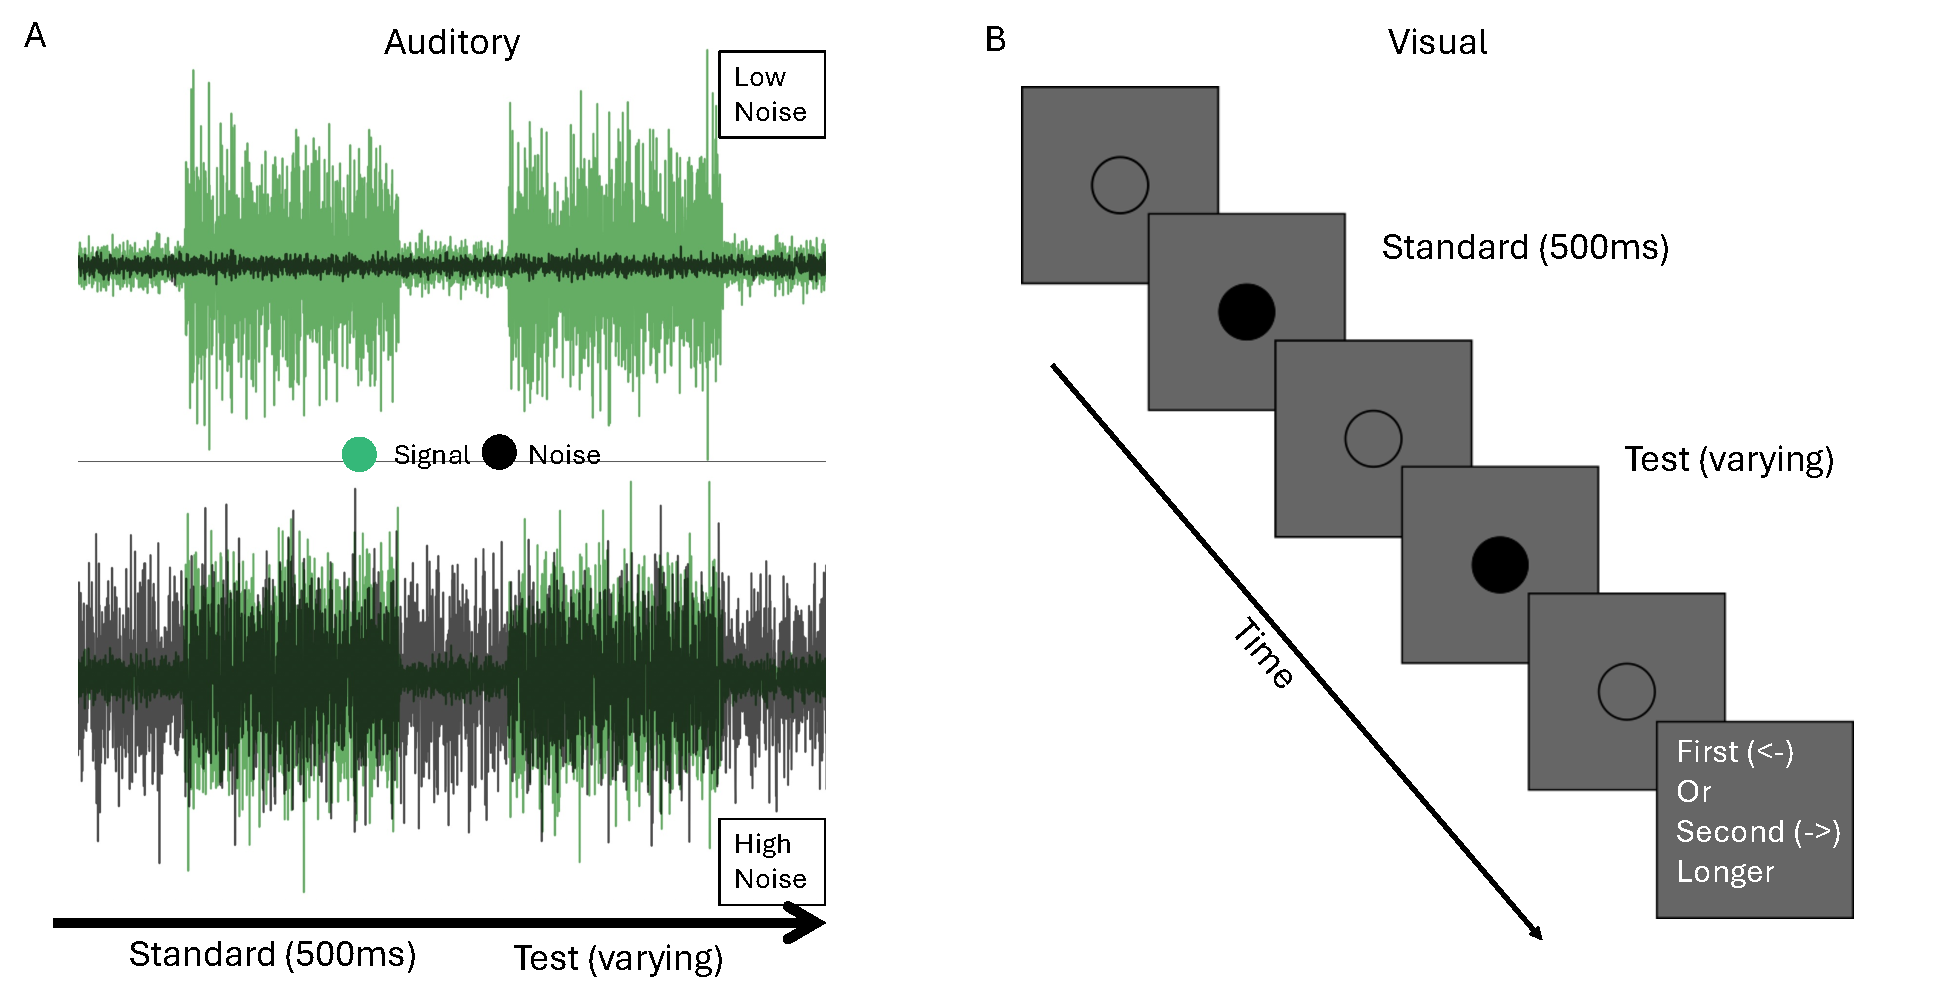
\includegraphics[width=1\linewidth]{assets/figures/unimodal_tasks_timeline.pdf}
    \caption{\textbf{Experimental stimuli and trial procedure.}
    Schematic illustration of the auditory and visual stimuli used in the duration-discrimination tasks. 
    \textbf{A} Example trials of the unimodal auditory task under the low (top) and high (bottom) auditory-noise conditions. In the low-noise condition, the auditory signal (bright green) is clearly distinguishable from the background noise (black). In the high-noise condition, signal and noise overlap substantially.
    \textbf{B} Trial timeline for the unimodal visual task. A disk outline remained visible throughout the trial to provide a stable visual reference. Each trial consisted of two sequentially presented stimulus durations (a standard and a test), separated by a short inter-stimulus interval (ISI). During each signal duration, the disk was filled (signal-on; shown dark), indicating the presence of the visual stimulus. Pre- and post-stimulus periods flanked the two intervals. The 500-ms standard and an adaptively varied test duration were presented in random order (standard-first order shown). Participants reported whether the first or second duration was longer.}
    \label{fig:unimodal_Timelines}
\end{figure}




\section{Methods}

\subsection{Participants}
We recruited twelve participants for the experiment, two of whom were the authors O.Y. and L.N., two were other lab members, while the rest were naive to the purposes of the experiment but experienced in psychophysical experiments. 
Testing was conducted in accordance with the ethical standards approved by the Institutional Review Board at New York University (protocol number FY2016--595). 
All participants provided informed consent prior to their involvement in the study and were compensated $\$15$ per hour for participation, except for the first author.

\subsection{Apparatus}

All experiments were conducted on a 21-inch CRT (Trinitron GDM-5402, Sony, Japan) with a refresh rate of 120~Hz and a spatial resolution of 800x600~pixels. The experiments were designed and executed using the Python PsychoPy package \citep{peirce2007psychopy}. The participants sat in a darkened room, approximately 60~cm away from the computer screen, with their head stabilized by a chin rest.

\subsection{Stimuli}

\subsubsection{Visual stimuli}

The visual stimulus was a black disk (0.07~cd/m\textsuperscript{2}) displayed in the center of the screen on a gray background (8.8~cd/m\textsuperscript{2}). The width of the disk was 3 degrees of visual angle. Throughout each trial the disk's black outline was continuously displayed. During the stimulus intervals, the inside of the circle changed from the background gray to black.

% \begin{figure}
%     \centering
%     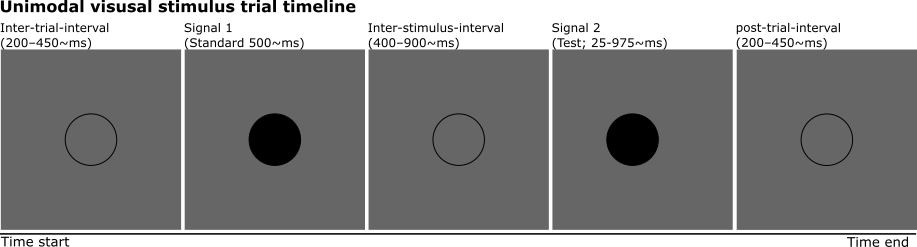
\includegraphics[width=1\linewidth]{assets/figures/visualTrialTimeline.png}
%     \caption{\textbf{Trial timeline and interval marking for unimodal visual task.}
%     A disk outline remained on screen throughout the trial to provide a stable background. During each interval (signal 1, signal 2) the disk was filled (signal-on; shown dark), indicating the visual ``duration'' to be judged. Pre- and post-stimulus periods flanked the stimulus intervals, which were separated by an inter-stimulus interval (ISI). On each trial, the 0.5-s standard and an adaptively varied test duration appeared in random order (the figure shows the standard-first order). Participants reported which interval was longer in duration.}
%     \label{fig:visualTimelineDiag}
% \end{figure}

\subsubsection{Auditory stimuli}

We adapted the stimuli from Hartcher and colleagues \citeyearpar{hartcher2014duration} and Shi and colleagues \citeyearpar{shi2013reducing} in which they created their stimuli by adding a pure-tone signal to a pink-noise background and manipulated duration uncertainty by varying the signal-to-noise ratio. Compared to their manipulation, in our stimulus, we generated white-noise waveforms for both the background and the signals. The background signal had a constant amplitude throughout the trial (Figure~\ref{fig:unimodal_Timelines}) The waveform for the signals had a low, non-zero amplitude before, between and after the pair of standard (fixed at 500ms) and test intervals (varying duration). During the standard and test intervals, the amplitude was increased. We then differentiated the signal from the background using different broadband filters to ensure that the signal was always detectable even when the background noise was louder than the stimuli. 

The auditory signals and the background noise were both filtered white-noise signals sampled at 48~kHz. Each interval's stimulus was a noise burst with increased amplitude modulated by a raised cosine (5~ms cosine ramp up, flat peak, cosine ramp down). The signal was embedded in a continuous background noise that spanned the entire trial. The signals waveform consisted of a pre-stimulus interval, first-interval stimulus, inter-stimulus interval, second-interval stimulus and post-stimulus interval, with the stimulus intervals defined by the raised-cosine amplitude envelope.

We manipulated auditory uncertainty by varying the relative amplitude of the continuous background noise with respect to the signal waveform before finally summing the two waveforms. In the low-noise condition, the background amplitude was approximately 0.1 times the stimulus amplitude, whereas in the high-noise condition it was approximately 1.2 times that amplitude. The final mixed waveform was then peak-normalized for playback.


To keep the ``signal'' perceptually distinct even with the high noise level, we applied different band-pass filters to the signal and background tracks. The background waveform was band-pass filtered with cutoffs at 10 and 610~Hz. The signal waveform (including the test and standard) was band-pass filtered from 150--775~Hz to make the stimuli more distinguishable from the background. The two waveforms were then summed to create the final stimulus. All filtering was implemented using second-order sections (SOS) Butterworth filters with a filter order of 4.

Auditory stimuli were calibrated using a Bruel \& Kjaer Type 2240 sound level meter positioned at the participant's head location. Sound levels were measured as A-weighted equivalent continuous levels (LAeq). The test and standard stimuli had an average intensity of approximately 70.5~dB~SPL (from the sum of the stimuli and background). In the low-noise condition, the continuous background noise (the sum of the background waveform and the non-stimulus signals waveform) was presented at 57.4~dB~SPL, yielding a signal-to-noise ratio (SNR) of approximately +13.1~dB. In the high-noise condition, the background noise was presented at 67.5~dB~SPL, yielding an SNR of approximately +2.9~dB. All sound intensities are reported as A-weighted levels.

To further characterize the stimulus structure, we additionally measured the sound levels of the individual stimulus components prior to mixing the background and signals waveforms. The background waveform averaged approximately 51.5~dB~SPL in the low-noise condition and 67.0~dB~SPL in the high-noise condition. For the signals waveform, the level during non-stimulus intervals (pre-stimulus, ISI, post-stimulus) was approximately 57.1~dB~SPL in the low-noise condition and 54.5~dB~SPL in the high-noise condition. During the stimulus intervals, levels increased to approximately 70.6~dB~SPL in the low-noise condition and 66.6~dB~SPL in the high-noise condition. These measurements confirm that the stimulus contained a clearly detectable signal embedded in background noise, with the signal interval producing a distinct increase in sound level relative to the baseline.





\subsection{Procedure}
Participants completed four experiments. First, they completed unimodal auditory and unimodal visual tasks, which were used to measure the uncertainty of duration perception for each modality. They carried out these two tasks in separate blocks at the beginning of the experiment to become familiar with the stimuli. 

After completing the unimodal tasks, participants completed the cross-modal baseline task, allowing us to measure and correct for perceptual bias between auditory and visual stimulus durations. We excluded one participant who showed a substantial perceptual bias (560 ms) toward visual duration in the high-noise auditory condition. 


Finally, participants performed the main experiment, which consisted of three sessions of approximately one hour each. Each session started with a flexible number of practice trials in which participants received feedback about the correctness of their answers until they felt comfortable with each task.

All tasks used a 2IFC design ("Which interval was longer?"). In each trial there was a standard and test stimulus. The order of standard/test stimuli was randomized across trials. Each trial comprised a pre-stimulus noise, first stimulus, an inter-stimulus interval (ISI), second stimulus, and a post-stimulus noise. Short breaks occurred every ~30 trials.

In the unimodal auditory, unimodal visual, and cross-modal experiments, the standard duration was fixed at 500~ms. In the bimodal experiment, the auditory component of the standard interval was always 500 ms. When audiovisual conflict was 0 ms, the visual component was also nominally 500~ms, but was adjusted based on the participant's audiovisual duration bias (see below). For non-zero conflict conditions, the visual duration was adjusted on each trial according to the conflict level (e.g., +250 ms conflict corresponded to a 750~ms nominal visual duration), while the auditory duration remained fixed at 500~ms.

Test stimulus duration was varied across trials according to adaptive staircase procedures (1-up/3-down or 1-down/3-up in the bimodal experiment). In the bimodal experiment, we compensated for each participant's modality-specific duration bias, measured in the cross-modal task, by adjusting the visual stimulus duration. This subject-specific correction ensured that auditory and visual components were perceptually matched in the test stimuli and in the zero-conflict standard condition. Below, we describe each experiment in detail.


The duration of the visual stimulus was perceptually matched to the auditory duration (the perceptual auditory duration bias, estimated using the data from the cross-modal task, was added to the duration of the visual stimulus) in both intervals. Then the conflict duration was added to the visual duration in the standard interval. Each trial consisted of a pre-stimulus interval (200--450~ms), the first stimulus (standard or test), an ISI (400-900~ms), the second stimulus (test or standard), and a post-stimulus interval (200-450~ms), forming one continuous audiovisual stimulus.


% \begin{figure}
%     \centering
%     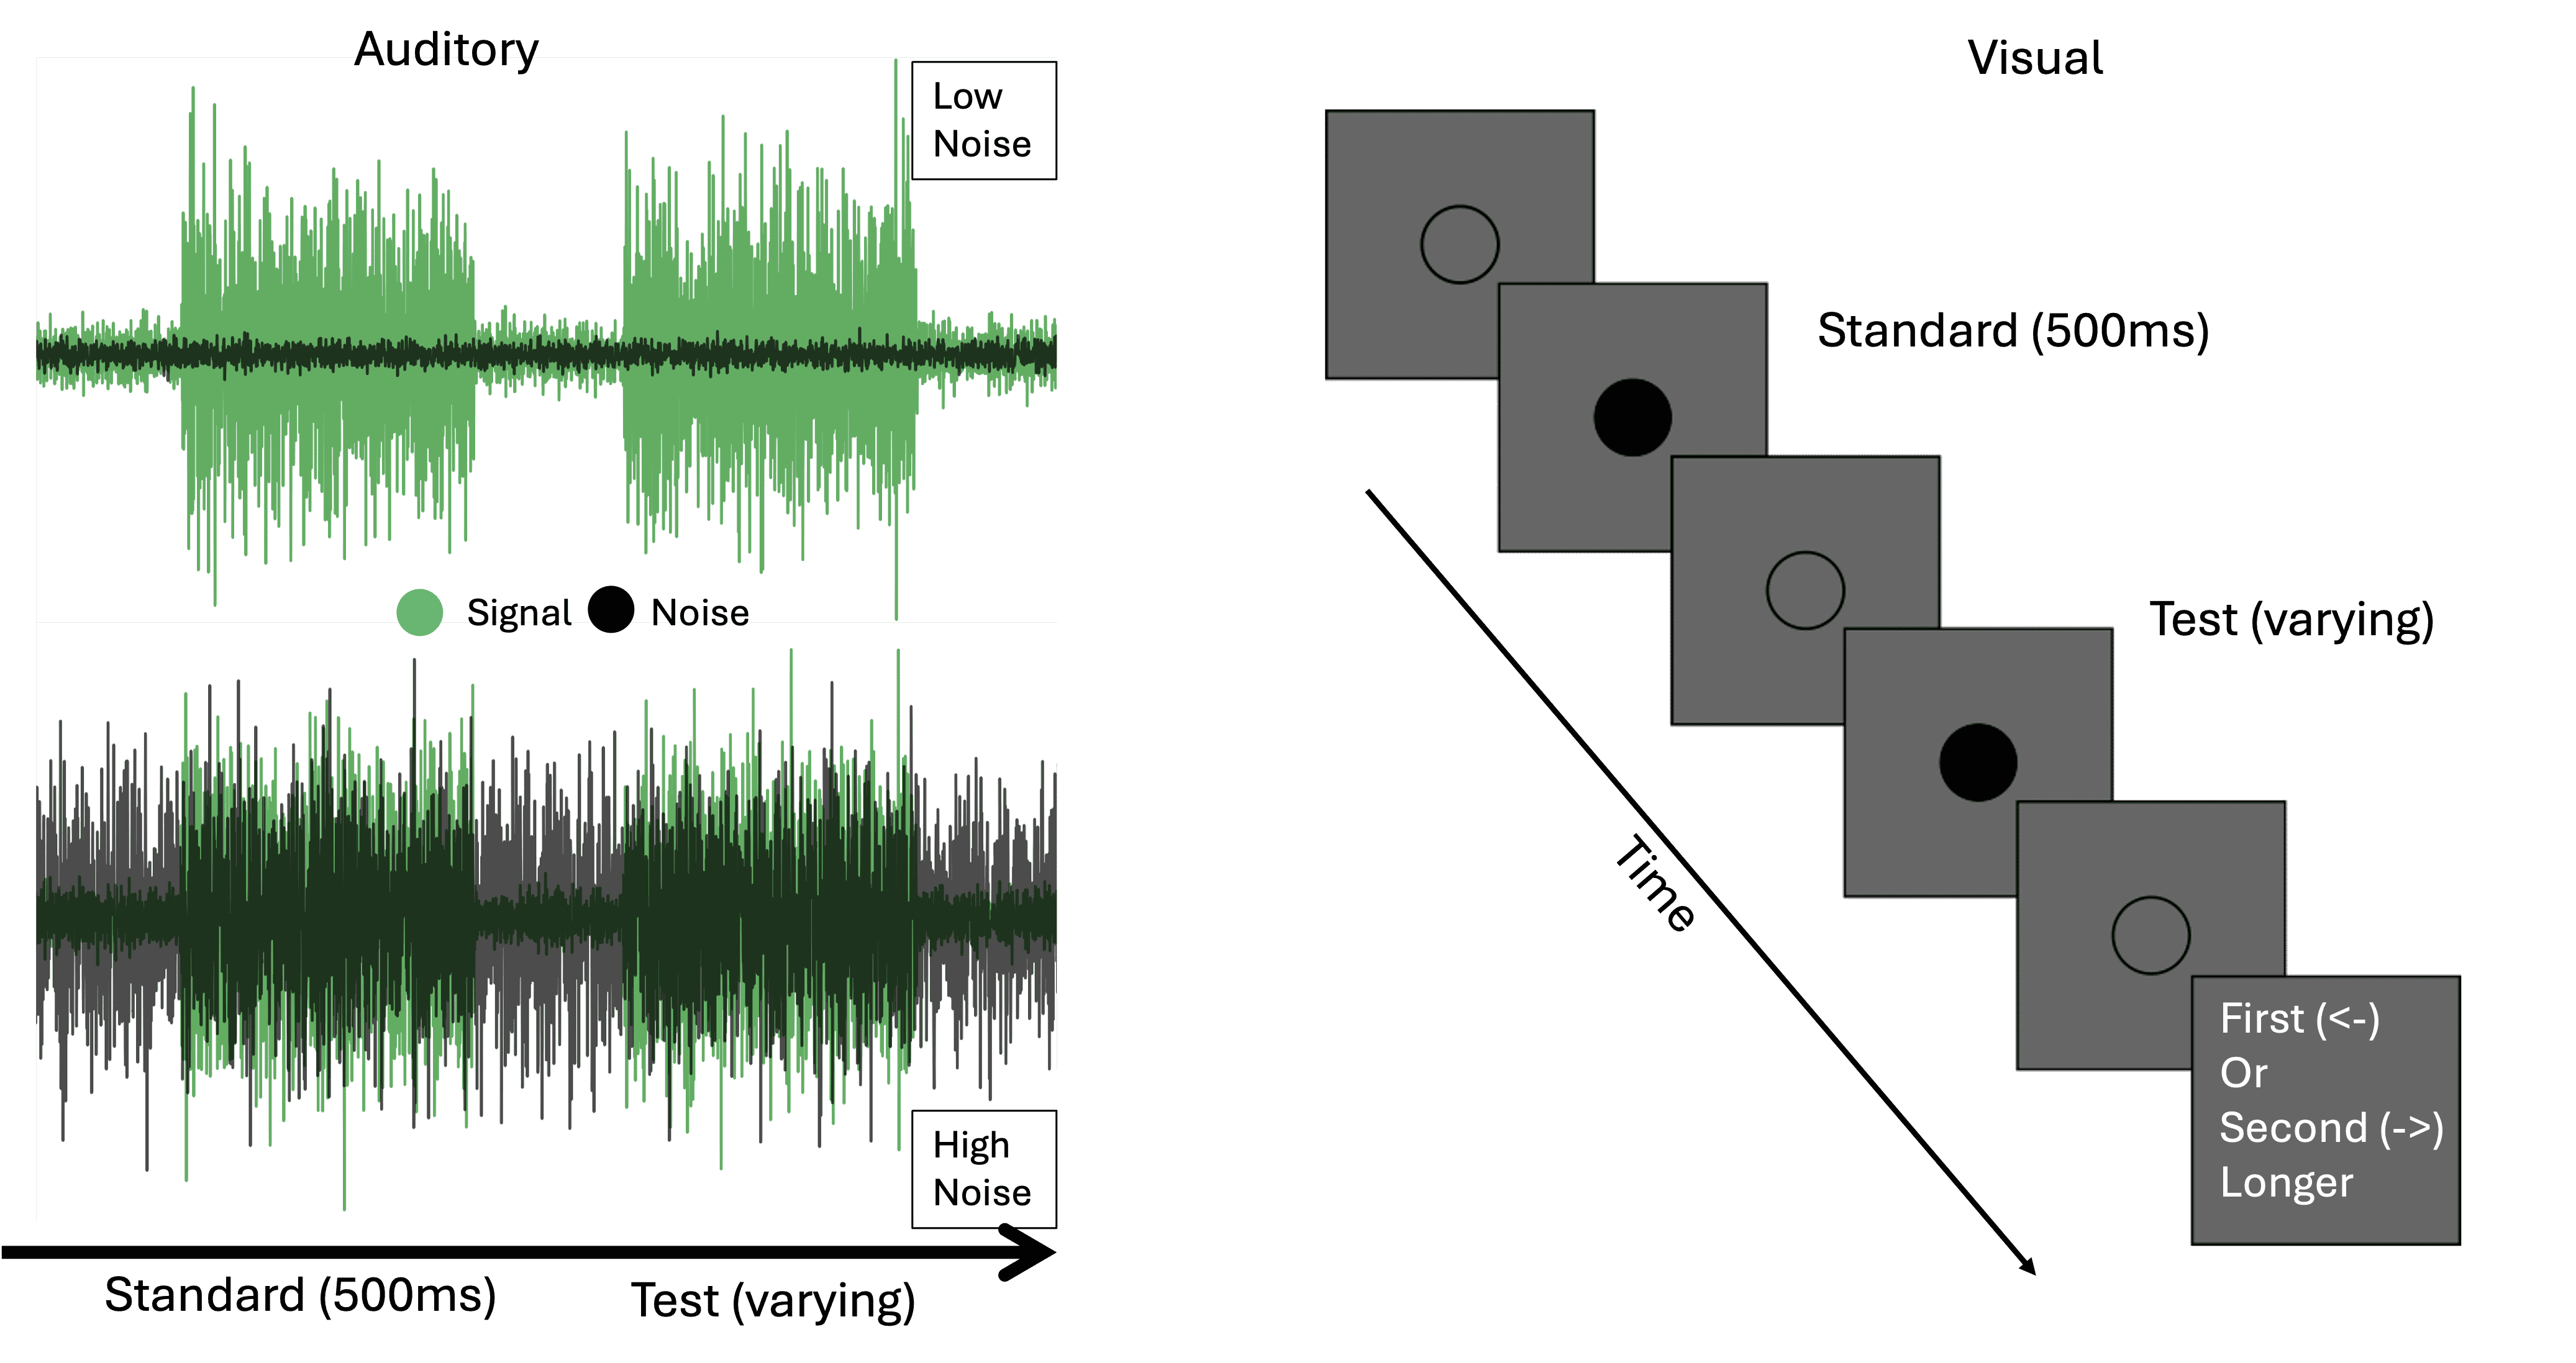
\includegraphics[width=1\linewidth]{assets/figures/unimodal_tasks_timeline.png}
%     \caption{\textbf{Experimental timeline and stimulus structure.}
% Schematic illustration of the auditory and visual stimuli used in the duration-discrimination tasks. \textbf{Left panel} showing the two example trial for the unimodal auditory experimental task trials. On the left panel top row the condition has low auditory noise (high signal to noise ratio) thus the signal (bright green) is much larger than the background noise. On the bottom on other hand it is a high auditory noise condition (low SNR) so that the signal and noise is mostly overlapped. For auditory taks stimulus waveform is generated by continuous background-noise (gray) spanning the entire trial (pre-stimulus, Interval 1, ISI, Interval 2, post-stimulus). The signal, a raised-cosine--gated noise burst whose flat-top equals the intended interval duration (shown in green), appears only during the two stimulus intervals. Background and signal were band-pass filtered over different frequency ranges, summed, and the sum was peak-normalized. Scaling of the background noise relative to the signal implements the SNR manipulation.\textbf{Right panel} on the other hand shows the trial timeline and interval marking for unimodal visual task. A disk outline remained on screen throughout the trial to provide a stable background. During each interval (signal 1, signal 2) the disk was filled (signal-on; shown dark), indicating the visual ``duration'' to be judged. Pre-and post-stimulus periods flanked the stimulus intervals, which were separated by an inter-stimulus interval (ISI). On each trial, the 0.5-s standard and an adaptively varied test duration appeared in random order (the figure shows the standard-first order). Participants reported which interval was longer in duration.}
%     \label{fig:unimodalTimelines}
% \end{figure}

\subsubsection{Unimodal baselines (Auditory only, Visual Only)}
In the unimodal tasks, 11 participants performed a 2IFC duration-discrimination task, in which  either two auditory durations (i.e., signals embedded on a background noise) or two visual durations (i.e., visual filled disks as signals) were sequentially presented. The auditory task lasted approximately 20~minutes, and the visual task lasted around 12~minutes. 

In both tasks, the standard stimulus duration was fixed at 500~ms. The duration of the test auditory stimulus varied (between 25 and 975~ms) from trial to trial. The waveform of an example stimulus in the low and high auditory-noise conditions is shown in Figure~\ref{fig:unimodal_Timelines}.

Test duration was determined  using four interleaved staircases: 1-Down 2-Up, 2-Down 1-Up, 3-Down 1-Up, and 1-Down 3-Up staircases of 70 trials each, resulting in a total of 280~trials for each unimodal task. We also included 14 trials with a large duration difference between the standard and test durations (+0.45s or - 0.45s) for each task. These trials allowed us to better estimate the lapse rate \citep{prins2012psychometric}.

% One of the 12 participants had a auditory duration discrimination threshold that was five times higher in the low SNR condition than in the high-SNR condition, and was excluded from further analysis.

\subsubsection{Cross-modal duration comparison}
In this task, participants compared the durations of one auditory and one visual stimulus. In each trial, the presentation order was precued. We split the experiment into 39 mini blocks of 10 trials. Before each mini block, we informed participants about the order of stimuli (e.g., "In this block the order of modalities will be: V->A") to orient their attention to both intervals and to understand the nature of the task. The order of stimulus presentation was randomized across mini-blocks.

% The point of subjective equality (PSE) extracted from psychometric functions was used to calibrate the perceptual biases in the main experiment. We incorporated the estimated bias in the main experiment. For example, if the visual bias was estimated to be $-$200~ms, we added $+$200~ms to the visual component of an audiovisual stimulus in the main experiment. This correction allowed the nominal ``zero-conflict'' condition to produce a PSE$\approx$0 for each participant.

\subsubsection{Main bimodal audiovisual conflict experiment}


In the main task, both the standard and test stimuli included visual and auditory durations. We introduced seven audiovisual duration conflicts, ranging from -250 to +250~ms (-250, -167, -83, 0, +83, +167, +250~ms) (Figure~\ref{fig:bimodalExpScheme}). We applied the conflict to both ends of the visual stimulus, i.e., half of the conflict magnitude extended the onset earlier and the other half extended the offset of the stimulus later. Likewise, visual PSE bias was subtracted from both ends of a visual stimulus so that a nominally zero-conflict stimulus had a visual component that was perceived as having the same duration as the auditory component. Also, note that this bias correction was applied to both the standard and test durations, while the visual-duration perturbation was only added to the standard stimulus.


Participants were asked to judge which interval had a longer duration based {\em only} on the auditory stimulus. Although participants were asked to judge the auditory stimulus, at the beginning of the experiment they were instructed to pay attention to both modalities and to maintain gaze at the screen even though they were not judging visual duration. We also included an audio icon to indicate that they needed to answer based on the auditory stimulus.



Each participant completed three sessions with different ranges of audiovisual conflict: (0, $-167$ to $250$ ms), ($-83$ to $167$ ms), and ($-250$ to $83$ ms). The order of sessions was counterbalanced across participants. As in the unimodal condition, easy lapse-rate trials were included in each experimental block (14 trials per condition; noise level $\times$ conflict). For each condition, participants completed four interleaved staircases (two 1-down--2-up and two 2-down--1-up), each consisting of 70 trials. Across all conditions and sessions, this resulted in a total of 2,156 trials for the main task.

\subsubsection{Staircases}

In all tasks, we measured discrimination thresholds using adaptive staircases, as described in each task section. Step-size reduction was applied after each staircase reversal. Specifically, whenever the staircase changed direction (from increasing to decreasing test duration, or vice versa), the step size was halved. Step-size reduction was applied only for the first two reversals; subsequent steps remained fixed.

The initial step size in the staircase procedure was defined as the duration difference percentage ($\Delta$) between the test and standard durations. At the beginning of the experiment, $\Delta$ was set to the largest negative value allowed, corresponding to $-95\%$ of the standard duration. Since the standard duration was 0.5~s, this yielded an initial test interval of $0.5 - 0.95 \times 0.5 = 0.025$~s. This value represents the shortest possible test interval used in the experiment.

The starting value of the staircase ($\Delta$) was set such that the resulting change in duration corresponded to approximately 25 ms for both auditory and visual cues. This ensured that the initial difference was clearly perceptible for participants.



\section{Results}

\subsection{Cue reliability}


% The auditory stimulus waveform is generated by continuous background-noise (gray) spanning the entire trial (pre-stimulus, Interval 1, ISI, Interval 2, post-stimulus). The signal, a raised-cosine--gated noise burst whose flat-top equals the intended interval duration (shown in green), appears only during the two stimulus intervals. Background and signal were band-pass filtered over different frequency ranges, summed, and the sum was peak-normalized. Scaling of the background noise relative to the signal implements the SNR manipulation.


% To characterize sensory precision, all participants completed two unimodal duration-discrimination tasks: one using auditory stimuli and the other using visual stimuli (Figure ~\ref{fig:unimodalTimelines}, for details see Methods and materials). For each task, we fitted log-normal psychometric functions to each participant's data using maximum-likelihood estimation. The log-normal observer model is more appropriate for duration data than cumulative Gaussian functions because it naturally incorporates Weber's law of scalar variability behavior and gives zero probability for negative durations, consistent with scalar timing theory. The psychometric model included three key parameters: lapse rate ($\lambda$), representing attentional lapses; discrimination parameter ($\sigma$), reflecting the steepness of the psychometric curve in log-space and duration sensitivity; and bias parameter ($\mu$), representing systematic over- or under-estimation of durations in log-space. In the log-normal model, the probability of judging the test duration as longer is given by: $$P(\text{``test longer''}) = \frac{\lambda}{2} + (1-\lambda) \cdot \Phi\left(\frac{\ln(t/s) - \mu}{\sigma}\right), $$ where $t$ and $s$ are test and standard durations, respectively, and $\Phi$ is the standard normal cumulative distribution function. In the unimodal experiments the bias parameter ($\mu$) was fixed at zero because, in our two interval forced choice (2IFC) design with randomized interval presentation, participants could not systematically bias their responses toward one interval over the other. Both the test and standard intervals were auditory stimuli of the same reliability (both high-noise or both low-noise). Thus participants can not have any bias towards perceiving one standard/test longer. Any bias would affect both test and standard stimuli equally and thus it makes sense to fix $\mu$ to zero. 

To measure sensory precision, all participants completed two unimodal duration-discrimination tasks: one auditory and one visual (Figure~\ref{fig:unimodal_Timelines}; see Methods for details). For each task, we fit log-normal psychometric functions to individual participant data using maximum-likelihood estimation.

The log-normal observer model is well suited for duration judgments, as it naturally captures scalar variability consistent with Weber's law and constrains duration estimates to be positive \citep{haigh2021role}. The psychometric function included two parameters: a lapse rate ($\lambda$), capturing stimulus-independent response errors, and a sensitivity parameter ($\sigma_v$ for the visual task and $\sigma_{a,l}$ and $\sigma_{a,h}$ for the low and high auditory-noise conditions), reflecting the uncertainty in sensory encoding (steepness of the psychometric function) in log-duration space.

We did not include a bias parameter ($\mu$) in the main analyses. In a symmetric two-interval, forced-choice (2IFC) design, any additive bias in perceived log-duration would affect both the standard and test intervals equally and therefore cancel in the comparison. Consequently, when  the standard ($t_s$) and the test ($t_t$) durations are identical, the model predicts $P(\text{``test longer''}) = 0.5$ by symmetry, and no bias term is theoretically required. 

Under this model, the probability of judging the test interval as longer than the standard is given by
\begin{equation}
P(\text{``test longer''}) = \frac{\lambda}{2} + (1-\lambda)\,
\Phi\!\left(\frac{\log(t_t)-{\log(t_s)}}{\sigma}\right),
\end{equation}
where $t_t$ and $t_s$ denote the test and standard durations, respectively, and $\Phi$ is the standard normal cumulative distribution function. Figure~\ref{fig:unimodal_data_fits} shows the unimodal duration-discrimination thresholds (Weber fraction; Panel A) and the psychometric-function fits (Panel B) for the auditory (high/low noise) and visual conditions.



\begin{figure}
    \centering
    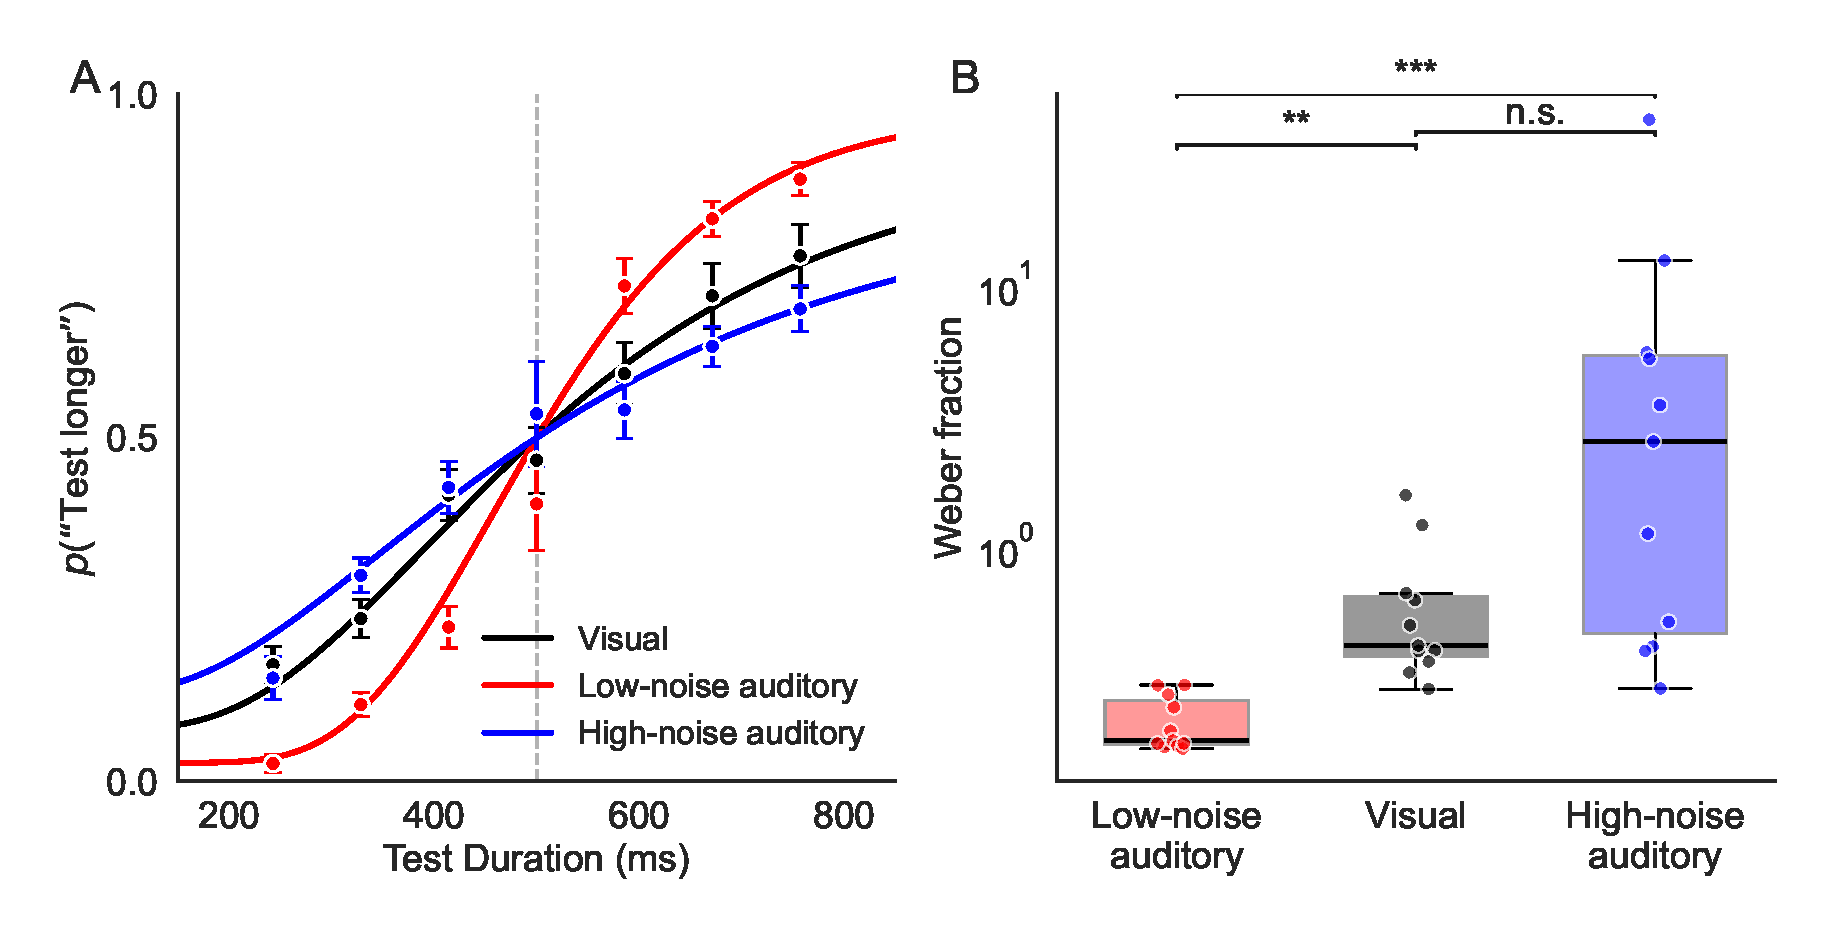
\includegraphics[width=1\linewidth]{assets/figures/psychometric_curves_publication.pdf}
    \caption{\textbf{Unimodal visual and auditory duration-discrimination psychometric functions.}   
     \textbf{B} Psychometric functions showing $p($``test longer''$)$ as a function of test duration, pooled across all participants and trials. Data points represent proportions calculated within duration bins; error bars indicate binomial standard errors. Solid lines show fitted log-normal psychometric functions. Red: low-noise auditory; black: visual; blue: high-noise auditory. Discrimination precision was highest for low-noise auditory, intermediate for visual, and lowest for high-noise auditory conditions.} \textbf{A} Unimodal discrimination thresholds expressed as Weber fractions, derived from log-normal psychometric fits, for the low-noise auditory (red), visual (black), and high-noisse auditory (blue) conditions. Each point represents an individual participant. Boxplots display the interquartile range (IQR; 25th--75th percentile), with the median indicated by the central line. Whiskers extend to the most extreme values within 1.5 $\times$ IQR of the first and third quartiles; values beyond this range are treated as outliers. Data points are horizontally jittered for visualization clarity.
    \label{fig:unimodal_data_fits}
\end{figure}

%%%%
The Friedman test and Wilcoxon signed-rank test analysis revealed significant effects of the auditory noise level on duration-discrimination precision. We conducted all analyses on the raw log-space noise estimates ($\sigma_v$, $\sigma_{a,l}$ and $\sigma_{a,h}$). However, for reporting purposes we converted these to just noticeable differences (JNDs) in milliseconds, defined as the minimum duration increment required to achieve 75\% correct performance and then to Weber fractions (WF). Given a fitted value of $\sigma$, the JND at 75\% accuracy is:
\begin{equation}
\text{JND} = t_s \left( \exp\left(z_{75}\sigma\right) - 1 \right),
\label{sigma2JND_eq}
\end{equation}
where $z_{75} = \Phi^{-1}(0.75)$ is the inverse cumulative normal value corresponding to 75\% correct.

We then computed the WF as the proportional threshold:
\begin{equation}
\text{WF} = \frac{\text{JND}}{t_s}.
\label{WF_eq}
\end{equation}


For the low- and high-noise auditory and visual conditions, the estimated Weber fractions were 0.18, 2.54, 0.42, respectively, with corresponding median JNDs of 92.5, 1271.8, and 212.7~ms. A Friedman test revealed a significant difference across conditions ($\chi^2(2) = 18.73, p < .001$; Figure~\ref{fig:unimodal_data_fits}), indicating that discrimination thresholds differed across the auditory (low- and high-noise) and visual conditions.


Pairwise comparisons were conducted using Wilcoxon signed-rank tests with Bonferroni correction ($\alpha = .0167$). $\sigma_{a,l}$ (low auditory-noise condition) was significantly lower than $\sigma_{a,h}$ (high auditory-noise condition; $W = 0$, $p < .001$). The value $W = 0$ indicates that, for every participant, the paired difference $\sigma_{a,h} - \sigma_{a,l}$ was positive, i.e., $\sigma_{a,l}$ was lower than $\sigma_{a,h}$ within all participants.  Moreover, $\sigma_{a,l}$ was significantly lower than $\sigma_v$ ($p < .001$). The difference between $\sigma_v$ and $\sigma_{a,h}$ was not significant after Bonferroni correction ($p = 0.18$).



\begin{figure}[H]
    \centering
    \includegraphics[width=1\linewidth]{assets/figures/cross_modal_timeline.pdf}
\caption{\textbf{Cross-modal duration-comparison trial structure.} Schematic of a single cross-modal trial. The trial consisted of two sequential stimuli (standard and test), separated by an inter-stimulus interval (dashed vertical lines indicate interval boundaries). \textbf{Top (auditory):} Continuous background noise was presented throughout the trial. A signal burst occurred during either the first or second interval. \textbf{Bottom (visual):} A disk outline was continuously visible. During the signal duration, the disk was filled. In this task, the visual stimulus was the standard, with a duration of 500-ms. The auditory test duration varied across trials. The auditory test and visual standard were presented in random order. }
    \label{fig:crossmodalDiag}
\end{figure}

\subsection{Modality-specific duration biases}

To estimate participants' inherent modality-specific biases in duration perception, we included a cross-modal duration-comparison task (Figure~\ref{fig:crossmodalDiag}). In this experiment, participants were presented with an auditory signal (embedded in continuous auditory noise) and a visual signal (a filled disk against an otherwise empty background). The presentation order of these stimuli was precued at the beginning of each mini-block of 10 trials. Participants reported which stimulus had the longer duration.

Psychometric fits revealed systematic biases in cross-modal judgments, with bias magnitude depending on auditory noise level (Figure~\ref{fig:crossModalData}). Under the low auditory-noise condition, the median point of subjective equality (PSE) shift was $-116$ ms, indicating that the auditory duration had to be physically shorter than the visual duration to be perceived as equal. A Wilcoxon signed-rank test confirmed that this shift differed significantly from zero ($W = 6, p = .014$). Under the high auditory-noise condition, the median PSE shift was $-73$ ms, indicating a reduced auditory bias. However, this shift did not differ significantly from zero. Together, these results indicate a reliable overestimation of auditory relative to visual duration in the low-noise condition, with a weaker bias under high auditory noise.


Given the systematic modality-specific biases observed in the cross-modal task, we estimated each participant's subjective auditory--visual duration bias and compensated for it in the bimodal experiment. Specifically, we adjusted the visual duration by adding half of the measured bias to the onset and half to the offset of the visual duration. This procedure preserved audiovisual synchrony while ensuring that, in the absence of added conflict, auditory and visual components were perceptually matched in duration. 


\begin{figure}[htbp]
    \centering
    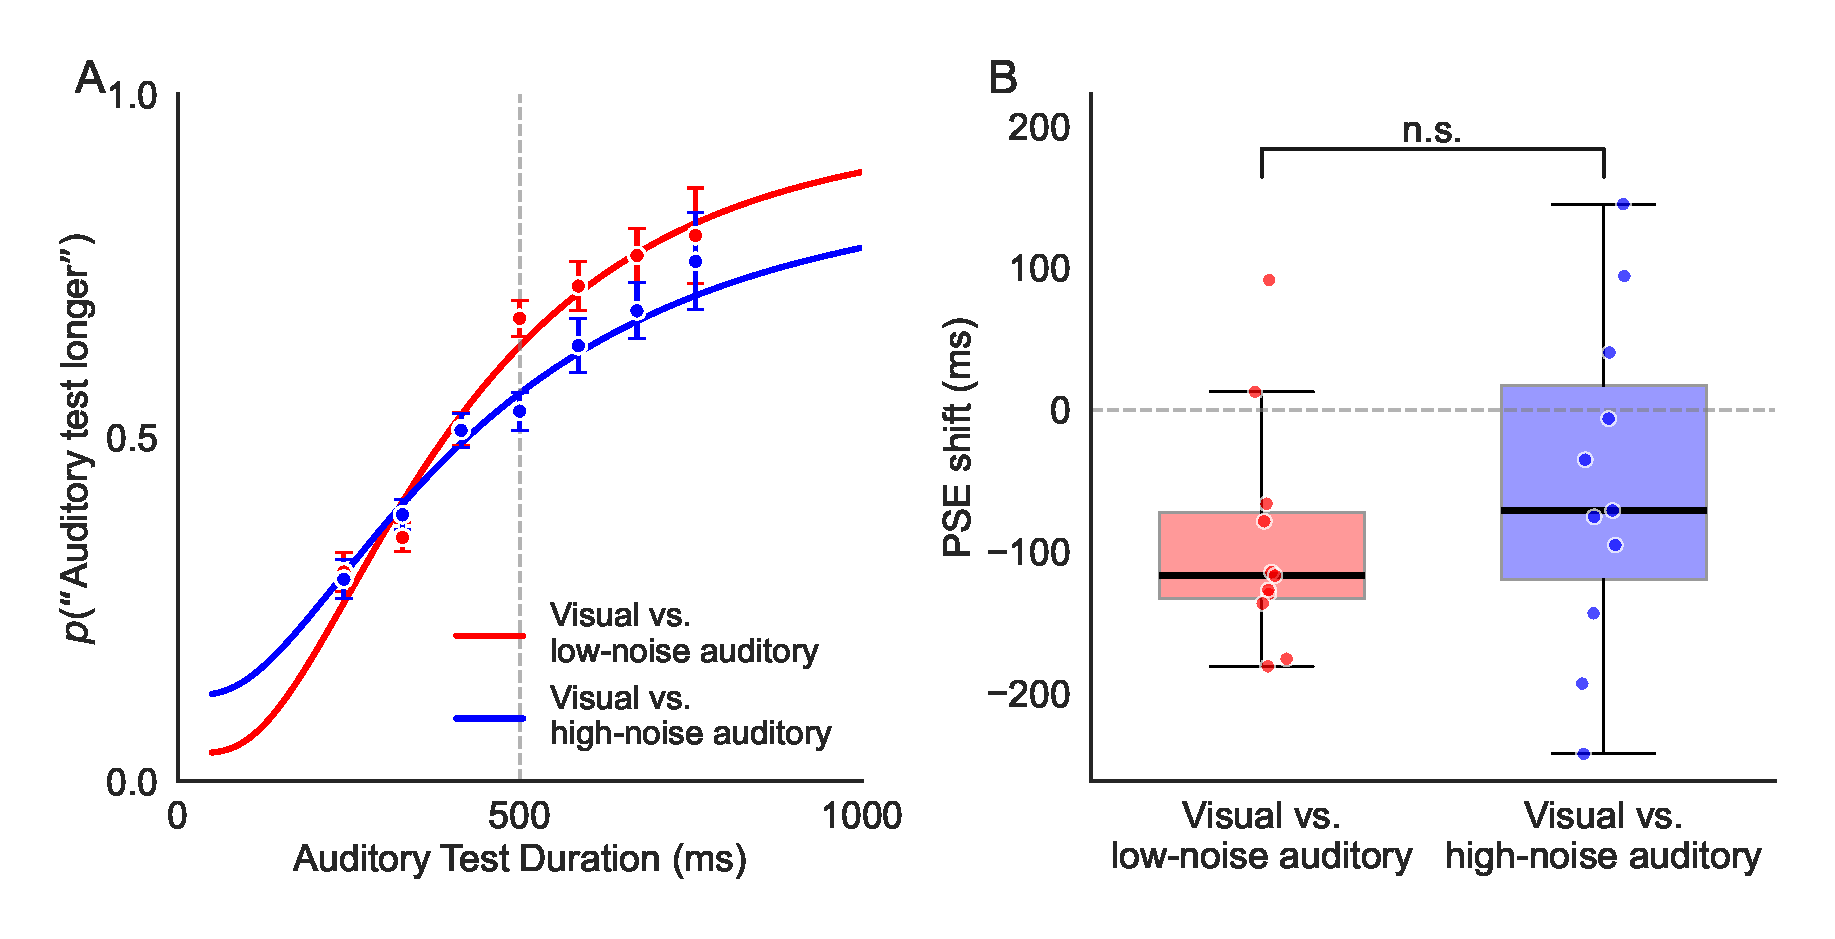
\includegraphics[width=1\linewidth]{assets/figures/psychometric_curves_crossmodal.pdf}
  \caption{ \textbf{PSE shifts and psychometric curve fits for the cross-modal duration comparison.} \textbf{A} Point of subjective equality (PSE) shifts for the low-noise auditory (red) and high-noise auditory (blue) conditions. Superimposed are the individual participant data points (horizontally jittered). The PSE shift is the difference between the standard duration (500~ms) and the auditory duration that is perceived as identical to the standard. \textbf{B} Psychometric functions (dots) and model fits (solid lines), showing $p($``auditory test longer''$)$. Binary data were grouped into 7 equally-spaced bins between 0 and 1000~ms (error bars: SEM).     For this plot we pooled the data across all participants then fitted with log-normal cumulative distribution functions (parameters: $\lambda$: lapse rate; $\mu$: PSE, $\sigma$: log-space noise). Solid lines show fit log-normal psychometric functions. 
  }
    \label{fig:crossModalData}
\end{figure}



\begin{figure}[H]
    \centering
    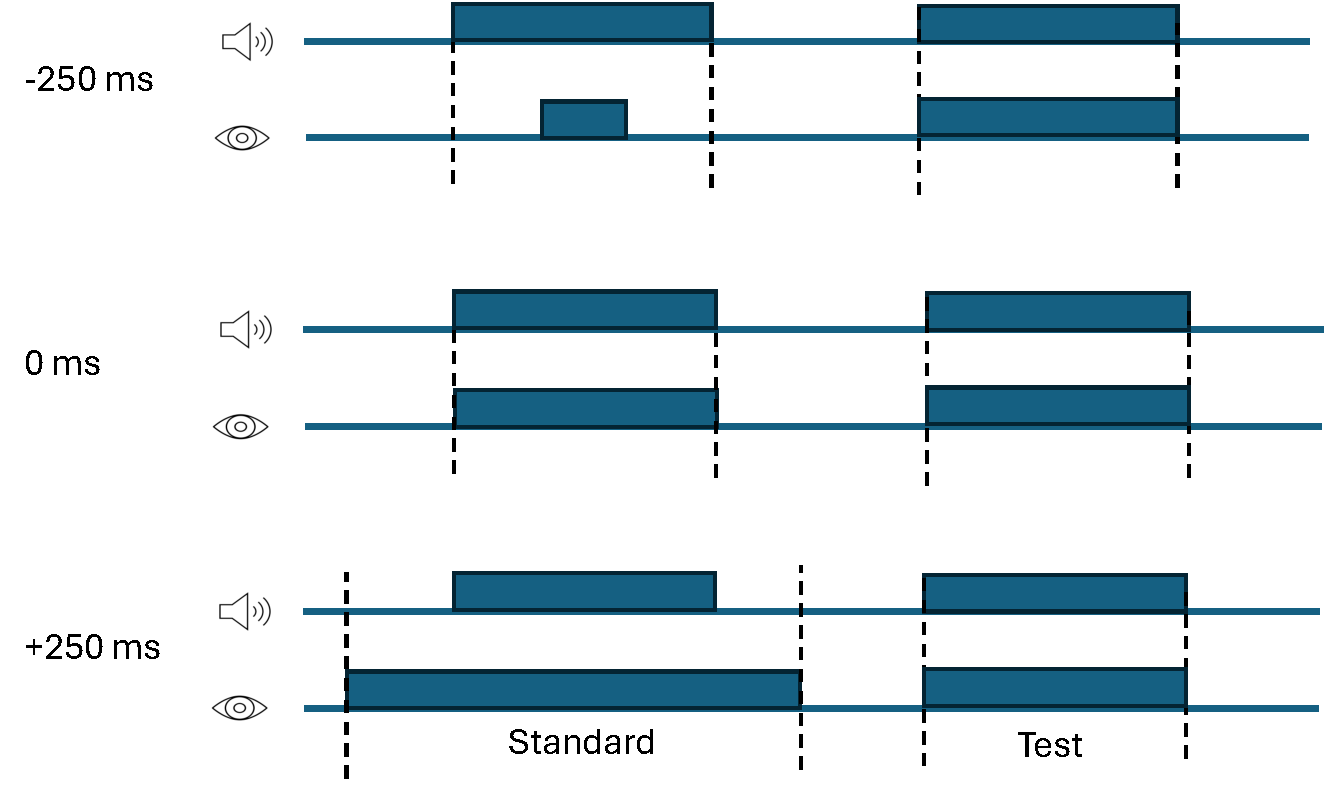
\includegraphics[width=1\linewidth]{assets/figures/bimodal_exp_scheme_1.pdf}
    \caption{\textbf{Audiovisual conflict in the bimodal experimental task.}
 Conflicts were introduced exclusively in the visual component of the \emph{standard} stimulus, while the auditory component remained unchanged. The top row shows an example negative-conflict ($-250$~ms), in which the visual duration of the standard stimulus was shorter than the auditory duration. Across trials, audiovisual conflict was randomly sampled from seven levels ranging from $-250$~ms to $+250$~ms. Note that the visual durations in both the standard and test stimuli were also corrected for the participant's audiovisual bias as estimated from the cross-modal task.}
    \label{fig:bimodalExpScheme}
\end{figure}

\subsection{Main experiment: Cue-conflict effects}

In the main bimodal experiment, participants were asked to judge which of two stimulus intervals was longer based solely on the auditory duration (Figure~\ref{fig:bimodalExpScheme}). Despite this instruction, participants' judgments were systematically influenced by the duration of the visual stimulus, especially under high auditory noise. 

To investigate how participants combined auditory and visual cues during duration judgments, we analyzed psychometric functions across varying levels of audiovisual conflict and auditory cue reliability. Figure~\ref{fig:psychometric_conflict_fits} shows the psychometric functions for each conflict level, separately for the low (left) and high (right) auditory-noise conditions. As the visual duration increased, the curves shifted horizontally toward longer durations, indicating that the task-irrelevant visual cue biased auditory duration judgments. This bias was more pronounced under the high-noise condition, qualitatively consistent with the predictions from reliability-weighted cue combination. Under low noise, psychometric functions showed smaller shifts, reflecting a stronger reliance on the auditory modality.

\begin{figure}
    \centering
    
\includegraphics[width=1\linewidth]{assets/figures/data_psychometric_functions_freeMuSigmaLambda_lognorm_clean.pdf}
 \caption{\textbf{Data and fitted psychometric functions in the bimodal experiment.} Fitted psychometric functions in the low auditory-noise condition. Each curve corresponds to one of seven audiovisual conflict levels ($-250$ to $+250$~ms). Dots show $p($``test longer''$)$ as a function of seven equally spaced test-duration bins. Data points are plotted at the centers of the bins, with dot diameter proportional to the number of trials within each bin. \textbf{B} Same as A, but for the high auditory-noise condition. Psychometric curves shift progressively with conflict magnitude, indicating stronger visual influence on perceived auditory duration under high auditory noise.}
    \label{fig:psychometric_conflict_fits}
\end{figure}

To quantify the results, we extracted the PSE from each psychometric curve and plotted it as a function of the conflict level (Figure~\ref{fig:conflict_pse}). Under the high auditory-noise condition, PSEs showed a nearly linear relationship with conflict magnitude. In contrast, under the low-noise condition, PSEs stayed close to zero, indicating reduced bias toward visual durations. The error bars reflect the Standard Error of the Mean across the 11 participant. We have also completed 1000 parametric bootstrapping for aggregated data. For each sample, we generated responses from the fitted psychometric function, refit the function, and computed the standard error of the resulting parameter estimates. Regression analysis confirmed a linear relationship between cue-conflict magnitude and PSE shifts. Under the high-noise condition, visual conflict magnitude showed a strong positive correlation with PSE shifts ($r$ = 0.963, $p$ $<$ 0.001), with a steep slope of 0.606~ms PSE change per 1 ms of visual conflict. In contrast, under the low-noise condition, the correlation remained strong ($r$ = 0.911, $p$ = 0.004), but had a much shallower slope of 0.144~ms per ms conflict. These results indicate that auditory duration perception was systematically biased toward the visual duration, and that the strength of this bias was modulated by auditory cue reliability.

\begin{figure}
    \centering
    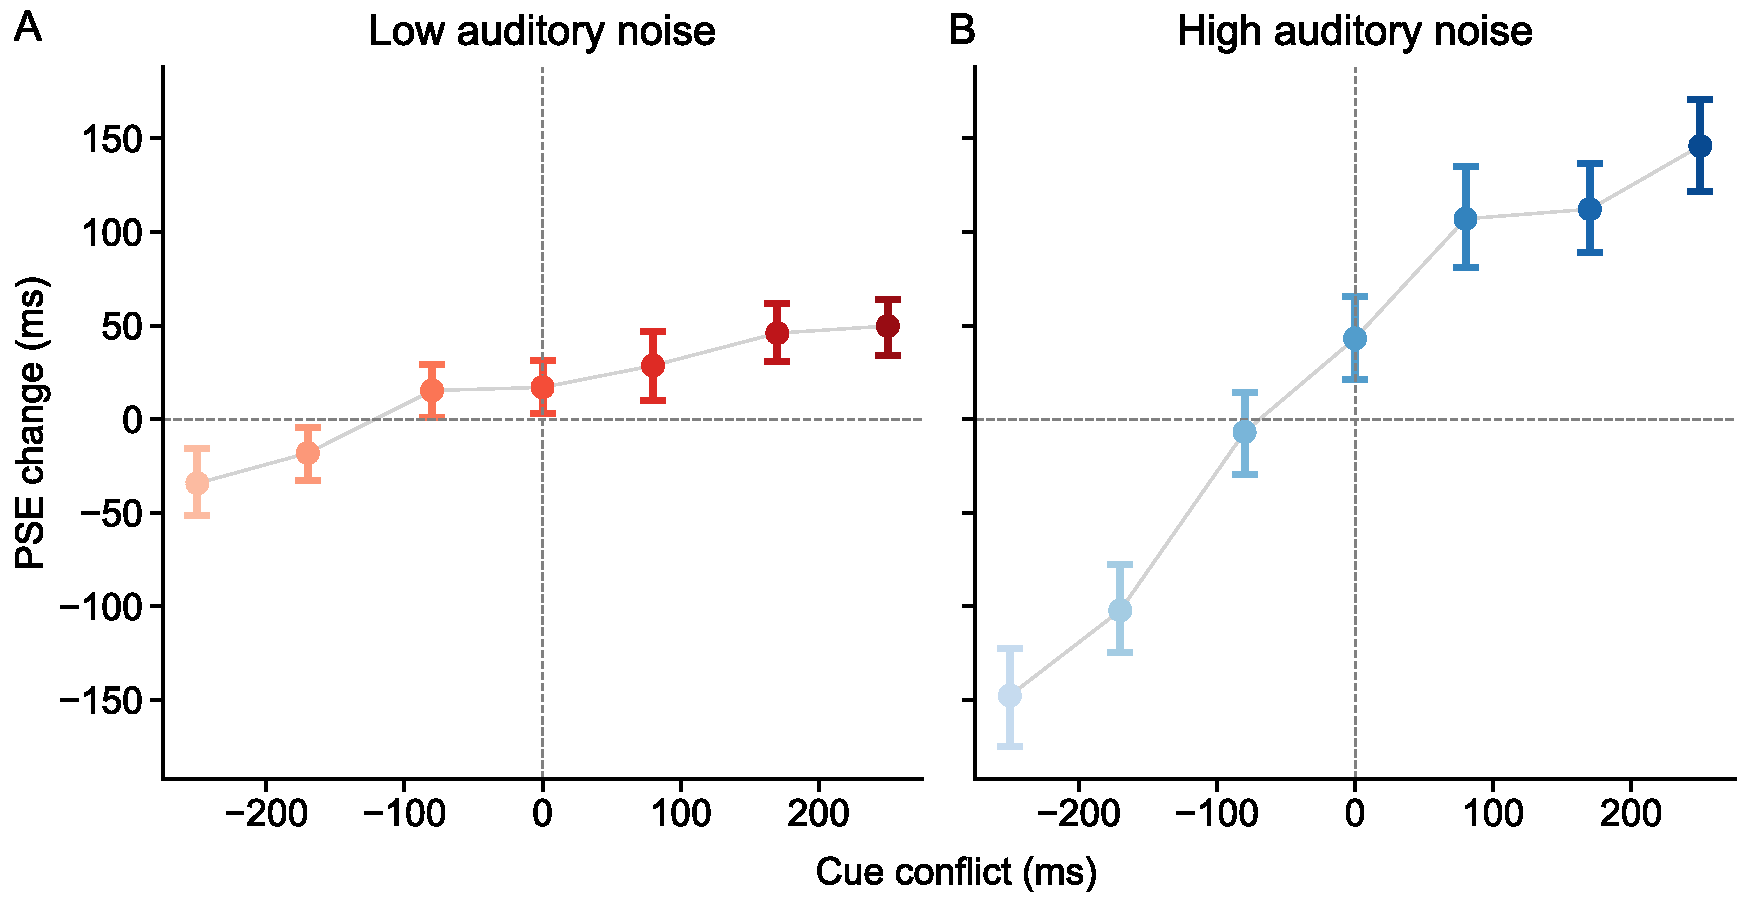
\includegraphics[width=1\linewidth]{assets/figures/pse_vs_conflict_all_1000_bootstrapped_ai.pdf}
\caption{\textbf{Effect of audiovisual conflict on perceived auditory duration.} Group-averaged point of subjective equality (PSE) estimates as a function of audiovisual duration conflict, shown separately for the low-noise auditory condition (\textbf{A}) and high-noise auditory condition (\textbf{B}). Each data point reflects the mean PSE of pooled data over 11 participants; error bars show SEM across participants. Under low noise, PSEs are more stable across conflict levels, suggesting auditory dominance.Under high noise, auditory duration judgments are pulled toward the visual duration.}
    \label{fig:conflict_pse}
\end{figure}


\section{Computational models}
To explain participants' behavior in the audiovisual duration-conflict task, we fit three models to the behavioral data. These models shared the same encoding process but differed in decoding strategy. Below, we describe the models' encoding process, followed by the decoding stage.

\subsection{Sensory encoding}
All models assumed that internal representations of auditory and visual durations are noisy. To capture Weber-like scaling of temporal uncertainty (scalar variability), we assumed that durations are encoded in logarithmic space with additive Gaussian noise: 

\begin{equation}
p(m_a \mid s_a) \sim \mathcal{N}(\log s_a,\sigma_a^2), \qquad
p(m_v \mid s_v) \sim \mathcal{N}(\log s_v,\sigma_v^2).
\end{equation}

\noindent Here, $s_a$ and $s_v$ denote stimulus durations in linear time units, whereas $m_a$ and $m_v$ represent internal measurements in log-duration space. Because encoding noise was Gaussian in log space, the implied distribution of internal measurements expressed in linear time is log-normal. This formulation naturally produced scalar variability, such that uncertainty scaled proportionally with stimulus duration. Scalar variability is a characteristic feature of perception of time and motivates this log-duration encoding. Thus, both encoding and decoding were performed in log-duration space \citep{killeen1987optimal, wittmann2009inner,ren2020ensemble}.


\subsection{Decoding strategy}
While all tested models shared the same encoding process, they differed in how encoded information is integrated and read out across sensory modalities. We considered three classes of integration and decision strategies: forced fusion, causal inference, and heuristic cue selection. We describe each of the three models next.  

% 
% start with fusion/integration model, followed by causal inference model, then by all heuristic models

\subsection{Forced fusion (Optimal cue integration)}
The forced-fusion model assumed that observers integrate auditory and visual signals for the auditory-duration judgment regardless of cue-conflict magnitude. Moreover, the integration is optimal, with each cue weighted by its reliability (Eq.~\ref{eq:forced_fusion}). 

This model can be viewed as causally inferring the probability of the two cues are 100\% originated from same source and so cues are always integrated regardless of cue-conflict magnitude. 

\subsection{Causal-inference model}
The Bayesian causal-inference model assumed that the observer first infers whether the auditory and visual cues arise from a common source by computing the posterior probability of a common source given the two cues' sensory measurements:
\begin{align}
p(C = 1 \mid m_a, m_v),
\label{eq:pc}
\end{align}
where $C = 1$ denotes a common cause. The observer then forms a posterior over the task-relevant variable (here, the auditory stimulus duration $s_a$) by averaging over two posteriors. The observer's posterior distribution over auditory duration is given by:
\begin{align}
p(s_a \mid m_a, m_v)
= {}& p(C = 1 \mid m_a, m_v)\,
      p(s_a \mid m_a, m_v,C=1) \notag\\
&+ p(C = 2 \mid m_a, m_v)\,
   p(s_a \mid m_a,C=2),
\label{eq:auditory_bimodal_estimate}
\end{align}
in which $p(C = 2 \mid m_v, m_a)$ indicates the posterior probability of separate causes. $p(s_a \mid m_v, m_a, C=1)$ and $p(s_a \mid m_a,C=2)$ specify the posteriors over $s_a$ under each causal scenario. The posterior probability of common cause computed as:


\begin{equation}
\begin{split}
p(C=1 \mid m_a, m_v)
=
\frac{
p(m_a, m_v \mid C=1)\, p_c
}{
\begin{aligned}
&p(m_a, m_v \mid C=1)\, p_c + p(m_a, m_v \mid C=2)\, (1 - p_c)
\end{aligned}
}.
\end{split}
\label{eq:posterior_common_cause}
\end{equation}

This model included the prior probability of common cause, $p_c$, which was fitted to the data. Likelihoods under the common-cause and separate-causes hypotheses were computed by marginalizing over the latent true stimulus durations using a bounded prior, following the standard formulation of Bayesian causal inference \citep{kording2007causal}. Full expressions, choice of prior distribution, and analytical derivations are provided in \hyperref[app:appendix]{Appendix}, specifically in \hyperref[causal_inf_equations]{the Bayesian causal-inference model subsection}.

We modeled the prior distribution of durations as a truncated uniform distribution over the range of stimulus durations presented in the experiment, $[t_{\min}, t_{\max}]$, providing finite support for the latent duration variable. 

Here the model assumed that participants inferred the stimulus duration based on the inferred causal relationship between the cues presented in the trial. It assumed that the observer started by inferring the posterior probability of both cues originating from a common cause by computing $p(C = 1 \mid m_a, m_v)$. Under this model, observers computed two estimates of the auditory stimulus duration, one based on both auditory and visual measurements, and another based on the auditory measurement alone. The final auditory duration estimate was a weighted average of these two separate estimates, given by:
\begin{align}
\hat S_{a}
= {}& p(C=1 \mid m_a,m_v)\,\hat S_{a,C=1} \notag\\
&+ \bigl(1 - p(C=1 \mid m_a,m_v)\bigr)\,
   \hat S_{a,C=2},
\label{eq:estimate_model_avg}
\end{align}
where $\hat S_{a,C=1}$ and $\hat S_{a,C=2}$ denote the estimates of the auditory stimulus under the common-cause and independent-causes assumptions, respectively.


The above computation yields an internal estimate of auditory duration for a single interval. In the present two-interval forced-choice task, the same inference process is applied independently to the standard and test intervals, producing estimates $\hat S_{\mathrm{std}}$ and $\hat S_{\mathrm{test}}$. The observer then compares the estimated durations of the test and standard intervals and responds ``test longer'' whenever

\begin{equation}
\hat S_{\mathrm{test}} > \hat S_{\mathrm{std}}.
\end{equation}

The predicted response probability is therefore

\begin{equation}
P(\text{``test longer''})
=
P\!\left(
\hat S_{\mathrm{test}}
-
\hat S_{\mathrm{std}}
>
0
\right),
\end{equation}

where the probability is obtained by marginalizing over the noisy sensory measurements through Monte Carlo simulation.


\subsection{Probabilistic cue switching}
We also considered a probabilistic cue-switching model, in which observers based their decision on either the auditory or the visual cue on each trial (see Methods). Instead of computing posterior probabilities of causal structure, this heuristic strategy selected a single cue stochastically: with fixed selection probability $p_v$, the decision was based solely on the visual estimate, and with probability $1 - p_v$, it was based solely on the auditory estimate. Thus, $p_v$ represents the probability of relying on the visual cue on a given trial. Despite its simplicity, the switching strategy can reproduce cue-integration--like patterns when responses are averaged across trials.




\subsection{Modeling results}

We first evaluate how well the models accounted for the shifts in PSE as a function of audiovisual cue conflict across the two auditory noise levels. We compared observed PSE shifts with predictions from three models: forced fusion, causal inference, and probabilistic cue switching. Sensory-noise parameters were fitted using the data from the bimodal experiment. 

Figure~\ref{fig:pseConflictModel} shows model fits to the PSE-shift data. All three models capture the overall pattern that perceived auditory duration was systematically biased toward visual duration and that the bias increased approximately linearly with audiovisual conflict magnitude. All three models also predict an overall larger bias under higher auditory noise. This convergence suggests that our data may be limited in the ability to adjudicate between these models. 

Causal-inference model typically predicts a non-linear breakdown of integration for large cue conflicts. Our data show only weak deviations from linearity. These deviations are more pronounced for large positive conflicts than for large negative conflicts, indicating an asymmetry in bias magnitude across the conflict range. This pattern suggests that, at the group level, observers do not exhibit the strong nonlinearity predicted by causal-inference model in which cue integration turns to cue segregation with increases in cue conflict. Instead, integration remains approximately linear within the tested conflict range. As a result, the behavioral signatures of causal inference are weak, limiting our ability to discriminate between causal-inference model and simpler integration or heuristic strategies with these data.



\begin{figure}
    \centering
    
\includegraphics[width=1\linewidth]{assets/figures/aggregated_mu_vs_models_freeMuSigmaLambda_sem_better_freeSigmaModel.pdf}
\caption{
Conflict-dependent biases in auditory duration perception. Point of subjective equality (PSE) shifts as a function of audiovisual conflict for the low auditory-noise condition (\textbf{A}) and high auditory-noise condition (\textbf{B}), averaged over 11 participants. Positive values indicate biases toward longer perceived auditory duration. Red and blue show empirical data (group mean $\pm$~SEM across 11 participants). Other lines indicate model predictions for forced fusion, causal inference, and probabilistic cue switching. The model predictions are jittered horizontally for readability. All model predictions were generated using sensory-noise parameters fitted using the bimodal data. For models, error bars reflect $\pm$~SEM across participant fits.}
\label{fig:pseConflictModel}
\end{figure}
\subsection{Model fitting and model comparison}
All models have a lapse-rate ($\lambda$) parameter, two auditory duration-noise parameters (one for each auditory-noise condition: $\sigma_{a,l}$ and $\sigma_{a,h}$), and one visual duration-noise parameter ($\sigma_{v}$). For models that incorporate causal inference, there is an additional parameter ($p_c$), which captures the prior probability of a common source. For the probabilistic cue-switching model, there are two additional parameters ($p_{v,l}$ and $p_{v,h}$) that specify the probability of switching (i.e., relying on vision rather than audition) in each of the two auditory-noise conditions.

We fit each model to each participant's data (from the two auditory-noise conditions jointly) using maximum-likelihood estimation. For each model, we computed the predicted probability of responding ``test longer'' for every stimulus condition via Monte Carlo simulation. Specifically, on each simulated trial, we drew noisy internal measurements of auditory and visual durations from the encoding model, applied the model's integration or decision rule to produce an estimate of the auditory stimulus, and then determined whether the test estimate was longer than the standard estimate. For each condition, that is, for each combination of auditory test duration, standard duration, cue conflict, and noise level, we simulated 2000 Monte Carlo trials (i.e., repeated draws of internal sensory measurements). For each Monte-Carlo trial we generated samples of the auditory and visual internal measurements according to the model's encoding-noise assumptions and determined the model's response for that trial. The predicted response probability for each condition was computed as the proportion of simulated trials for that condition for which the model observer judged the test duration as longer. The log-likelihood of each model was then computed using the binomial likelihood of the observed responses given the predicted probabilities across all conditions. Parameter bounds were chosen based on plausible ranges for sensory noise and lapse rates. In causal-inference model, the prior over stimulus duration was assumed to be uniformly distributed over the range of test durations presented for each participant. Parameters were estimated by minimizing the negative log-likelihood using Bayesian Adaptive Direct Search \citep{acerbi2017practical}. To reduce the risk of local minima, the optimization was repeated from 10 random initial parameter values.

Sensory-noise parameters were fitted using the data from the bimodal task, because effective noise may differ between unimodal and bimodal contexts due to attentional allocation and cross-modal interactions \citep{badde2020modality}. To ensure robustness, we also evaluated all models using sensory-noise parameters estimated using the psychometric function fits to the unimodal-task data. The results using these parameter estimates were qualitatively consistent (Figure~\ref{fig:AppendixConflictPSE_unimodal_fits}).


%%% Changed this paragraph
We evaluated model performance using the Akaike Information Criterion (AIC) at the individual participant level. Model comparison was performed under two assumptions about sensory noise: (a)~sensory noise fixed to values estimated from unimodal task data and (b)~sensory noise fitted directly using the bimodal data (Figure~\ref{fig:modelComparison}). To summarize model preference at the group level, we simply added up each participant's $\Delta$AIC relative to the forced-fusion model across the 11 participants; a negative total means a model had a lower overall AIC than forced fusion (Figure~\ref{fig:sumDeltaAIC}). We attached 95\% confidence intervals to these totals by resampling participants with $10{,}000$ bootstrap resamples. To confirm that Monte-Carlo evaluation noise in the simulated likelihood did not drive the comparison, we additionally re-evaluated each fitted model's log-likelihood at its maximum-likelihood parameters under 20 independent random seeds (using the same 2000 Monte-Carlo trials per condition) and took the standard deviation of the resulting per-participant AIC as a Monte-Carlo noise floor. This noise floor was small (median $1.6$ and $1.9$ AIC points for the fixed- and free-noise analyses, respectively), and all fits reproduced their stored log-likelihoods within it.

% Reproducibility: bootstrap = modelComparisonTable_threeModels.ipynb, section 4 (bootstrap_aic, plot_mean_delta_aic) -> meanDeltaAIC_threeModels.pdf; Monte-Carlo noise floor = co           +mpute_aic_noise_floor.py (cache aic_noise_floor_seeds.json), notebook section 4b.


% We evaluated model performance using the Akaike Information Criterion (AIC) at the individual participant level. Model comparison was performed under two assumptions about sensory noise: (a)~sensory noise fixed to values estimated from unimodal task data and (b)~sensory noise fitted directly using the bimodal data (Figure~\ref{fig:modelComparison}).

Consistent with the observation that all models captured the data reasonably well (Figure~\ref{fig:pseConflictModel}), model comparison revealed only small differences in fit quality across integration strategies. Below, we report model-comparison results under two conditions: sensory-noise parameters were (1)~fixed to values estimated from the unimodal experiment, or (2)~treated as free parameters and fit directly to the bimodal data.

\subsubsection{Fixed sensory noise}
In this analysis, we assume that sensory noise is identical for unimodal and bimodal stimuli. Thus, we estimated the noise parameters using the data from the unimodal duration-discrimination tasks, and then used those estimates when fitting the data from the bimodal task. Figure~\ref{fig:modelComparison}A shows the participant-level $\Delta$AIC values, computed as the difference between the each models' AIC for each participant and the AIC values of the Forced fusion model. For most participants (8 out of 11), the probabilistic cue-switching model achieved the lowest $\Delta$AIC among the candidate models, indicating that it provided the best trade-off between goodness of fit and model complexity. The Bayesian causal-inference model was the best-fitting model for the remaining three participants. The forced-fusion model did not achieve the lowest $\Delta$AIC for any participant.

At the group level, the summed $\Delta$AIC values across participants yielded the same pattern, with the probabilistic cue-switching model overall performing the best (Figure~\ref{fig:modelComparison}A right panel). 


\begin{figure}
    \centering
    
\includegraphics[width=1\linewidth]{assets/figures/modelComparison_threeModels_heatmap.pdf}
 \caption{
    \textbf{A} Model comparison assuming sensory-noise parameters fixed to values estimated from the unimodal tasks. \textbf{B} Model comparison when sensory-noise parameters were additionally fit to the bimodal data. Left panels show participant-level $\Delta$AIC values for each model, computed relative to the forced-fusion model (the baseline column, which is therefore identically zero); negative values (blue) indicate a better fit than forced fusion. Rows correspond to participants and columns correspond to models, and the best-fitting model (lowest AIC) for each participant is outlined. Right panels show the sum of these $\Delta$AIC values across participants for each model, providing a group-level comparison. When sensory-noise parameters were fixed (A), the probabilistic cue-switching model provided the best fit for 8 of 11 participants. When the sensory-noise parameters were fit directly to the bimodal data (B), the cue-switching model provided the best fit for 6 of 11 participants.
    }
    \label{fig:modelComparison}
\end{figure}

\subsubsection{Free sensory noise}

When sensory-noise parameters were fitted using the bimodal data, model comparison revealed substantially weaker separation between candidate models (Figure~\ref{fig:modelComparison}B). Participant-level $\Delta$AIC values showed considerable overlap between models, indicating that multiple integration strategies provided similarly good fits once sensory noise was allowed to vary.

The probabilistic cue-switching model provided the best fits for the largest number of participants (6 out of 11; Figure~\ref{fig:modelComparison}B). At the group level, it also yielded the lowest summed $\Delta$AIC across participants. However, the individual $\Delta$AIC values were very low, suggesting limited discriminability between integration strategies under this assumption.


%%%% ----- Bootstrapped AIC

\subsubsection{Group-level model comparison and its reliability}
To summarize models across participants, we summed each participant's $\Delta$AIC relative to the forced-fusion model: a negative sum means the model had a lower total AIC than forced fusion across the group, and the further below zero, the stronger the group-level preference (Figure~\ref{fig:sumDeltaAIC}). Under fixed sensory noise, both the probabilistic cue-switching model (summed $\Delta$AIC $= -448$, 95\% CI $[-764,\,-173]$) and the causal-inference model ($-204$, $[-471,\,-28]$) fit better than forced fusion, with cue switching preferred overall; both confidence intervals fell entirely below zero. Under free sensory noise, the same ordering held, but the totals were much smaller and no longer reliable (cue switching $-34$, $[-73,\,+1]$; causal inference $-1$, $[-17,\,+14]$), with both confidence intervals overlapping zero.

This lack of separation under free sensory noise is not an artifact of Monte-Carlo evaluation noise. The per-participant AIC noise floor (median SD $1.9$ AIC points) was comparable in magnitude to the per-participant $\Delta$AIC itself, so individual-participant model assignments are unreliable in this regime; averaging across the 11 participants, however, reduced the Monte-Carlo contribution to below $1$ AIC point. The null result therefore reflects genuine between-participant variability in model preference rather than simulation noise.


%%% --- adding this: random-effects Bayesian model selection (model frequencies / exceedance probability) ---

% Reproducibility: modelComparisonTable_threeModels.ipynb, section 6 (Random-effects Bayesian model selection); prints E[r], XP, PXP, BOR; figures pxp_threeModels_freeSigma.pdf / pxp_threeModels_unimodalSigma.pdf.

We complemented these criteria with random-effects Bayesian model selection, which estimates the frequency of each model in the population and is robust to outlying participants \citep{stephan2009bayesian,rigoux2014bayesian}. Probabilistic cue switching was the most frequent model under both assumptions about sensory noise, with an estimated model frequency of $0.65$ and an exceedance probability of $0.93$ under fixed sensory noise, and $0.46$ (exceedance probability $0.68$) under free sensory noise. Consistent with the small $\Delta$AIC differences, however, the Bayesian omnibus risk was high ($0.87$ and $0.77$, respectively), indicating that the candidate models cannot be confidently separated at the group level; the protected exceedance probabilities were correspondingly modest (approximately $0.41$ for cue switching in both analyses).
%%% --- end added section ---


\begin{figure}[H]
    \centering
    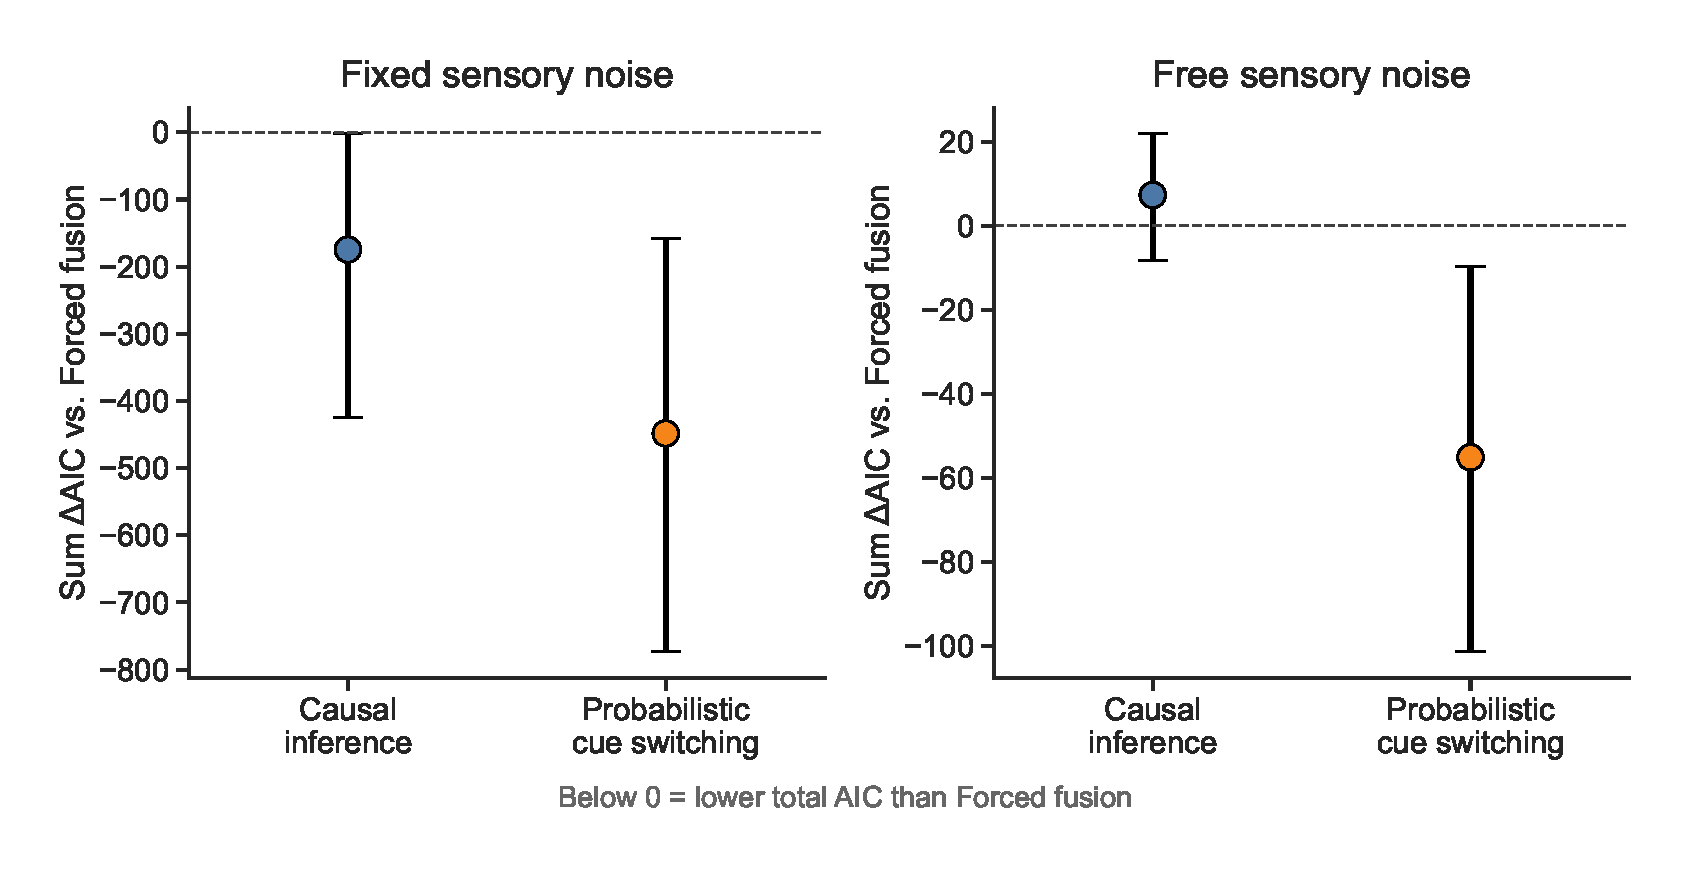
\includegraphics[width=0.8\linewidth]{assets/figures/sumDeltaAIC_threeModels.pdf}
    \caption{\textbf{Group-level model comparison: summed $\Delta$AIC.} Sum of the per-participant $\Delta$AIC relative to the forced-fusion model (the baseline, fixed at $0$ and not shown) under fixed (left) and free (right) sensory noise. Each colored point is the total across the 11 participants for one model, with 95\% confidence intervals from $10{,}000$ participant bootstrap resamples. Values below the dashed zero line indicate a lower total AIC, i.e. a better fit, than forced fusion. Under fixed sensory noise, the probabilistic cue-switching and causal-inference models fit clearly better than forced fusion (intervals below zero); under free sensory noise the totals are much smaller and the confidence intervals overlap zero.}
    \label{fig:sumDeltaAIC}
\end{figure}

%%%% ------



%%% --- adding this: switching-probability mechanism (figure + paragraph) ---
% Reproducibility: make_switching_prob_figure.py -> switching_probability_by_noise.{pdf,png}; reads model_fits/<pid>/<pid>_switchingFree_LapseFix_sharedPrior_fit.json (p_v,low = fittedParams[3], p_v,high = fittedParams[5]).

\subsubsection{Switching probabilities increase with auditory noise}
Beyond model comparison, the parameters of the favoured model were themselves consistent with the cue-switching account. The fitted probability of relying on the visual duration ($p_v$) increased markedly with auditory noise, rising from a group mean of $0.17$ under low auditory noise to $0.51$ under high auditory noise (Wilcoxon signed-rank test, $p = 0.003$; an increase in $10$ of $11$ participants; Figure~\ref{fig:switchingProb}). Thus, observers were estimated to rely on the visual duration roughly half of the time when auditory reliability was low, but only about one in six trials when it was high, providing a concrete and consistent mechanism for the noise-dependent visual bias.

\begin{figure}[H]
    \centering
    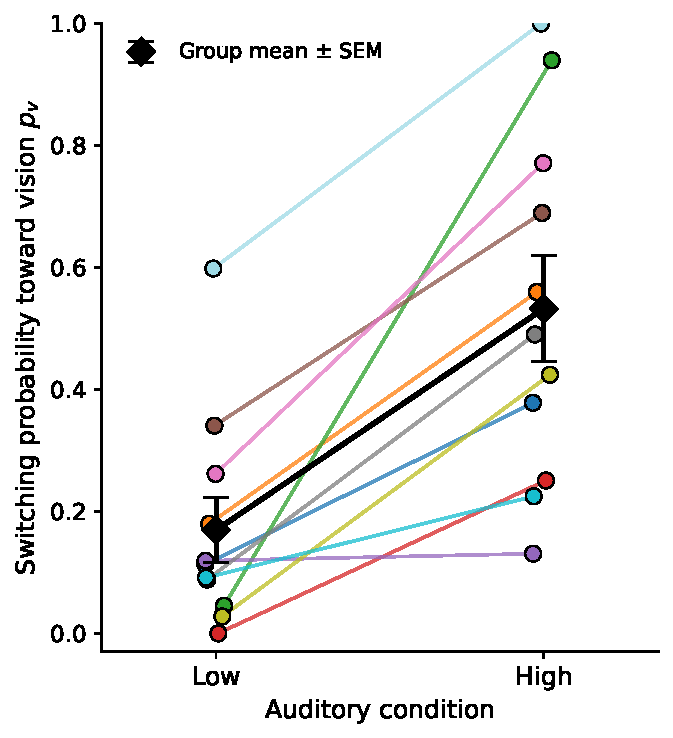
\includegraphics[width=0.55\linewidth]{assets/figures/switching_probability_by_noise.pdf}
    \caption{\textbf{Fitted switching probabilities increase with auditory noise.} Each thin line shows one participant's fitted probability of relying on the visual duration ($p_v$) in the low- and high-auditory-noise conditions, estimated from the probabilistic cue-switching model (free sensory-noise fits). The probability of relying on vision increased with auditory noise in $10$ of $11$ participants (group means $0.17 \rightarrow 0.51$; Wilcoxon signed-rank $p = 0.003$). Black line show group means $\pm$ SEM.}
    \label{fig:switchingProb}
\end{figure}
%%% --- end added section ---

\subsubsection{High sensory-encoding noise limits model discriminability}
To explain the lack of evidence for causal inference even at large audiovisual cue conflicts, we recovered the posterior probability of common cause $P(C=1 \mid m_a, m_v)$ across conflict levels using each participant's fit parameters.

Figure~\ref{fig:posterior_conflict} shows $P(C=1 \mid m_a, m_v)$ for an example participant. Across all conflict levels and auditory-noise conditions, the posterior probability of common cause remained relatively high (i.e., above 0.5), a pattern that was maintained for all participants (Figure~\ref{fig:posterior_individual}). This is due to the large sensory encoding noises estimated from the data. Specifically, when sensory encoding noise is high, even substantial physical conflicts produce overlapping measurement distributions, yielding consistently high posterior probability of common cause. This indicates that, the observer's fitted parameters are consistent with treating the auditory and visual signals as originating from a common source regardless of the imposed conflict.

This analysis reveals why causal-inference model and forced-fusion models produced similar predictions in our experiment. Given the estimated sensory-noise parameters, the posterior probability of common cause never dropped low enough to produce substantial segregation of cues. The observer's inference remained dominated by the common-cause hypothesis across the entire conflict range, resulting in near-linear, fusion-like behavior. Within the conflict range examined here, competing models predict largely overlapping, noisy psychometric patterns, imposing a fundamental limit on model identifiability rather than reflecting insufficient data or model distinguishability.

\begin{figure}
    \centering
    
\includegraphics[width=0.8\linewidth]{assets/figures/manuscript_posterior_p2_v3.pdf}
  \caption{\textbf{Posterior probability of common cause across conflict levels.}
    Log likelihoods and posterior probability of common cause for an example participant, plotted as a function of audiovisual duration conflict. Top row: low-auditory-noise condition; bottom row: high-auditory-noise condition. Left column: log likelihood of the measurements under a common cause, $\log P(m_a, m_v \mid C{=}1)$ (blue) and under separate causes, $\log P(m_a, m_v \mid C{=}2)$ (red), plotted on the same axes so that their relative magnitudes can be compared directly. Right column: Posterior probability of common cause, $P(C{=}1 \mid m_a, m_v)$, with the dotted line marking the fitted prior $p_c$. All quantities were computed via Monte Carlo simulation (500 samples per conflict level) using participant-specific sensory-noise estimates ($\sigma_{a,l}$, $\sigma_{a,h}$, $\sigma_v$) and common-cause prior ($p_c$) obtained from the log-normal causal-inference model fit.}
    \label{fig:posterior_conflict}
\end{figure}


\section{Discussion}
In this study, we investigated how humans infer duration under conflicting audio and visual cues with varying levels of sensory uncertainty. Previous work has shown that audiovisual duration cues can be integrated in a statistically optimal, reliability-weighted manner \citep{shams2005sound,hartcher2014duration}. Extending this framework, we asked whether such integration is flexibly modulated by causal inference, as observed in audiovisual spatial-localization tasks where large cue conflicts induce non-linear breakdowns of integration \citep{kording2007causal, badde2021causal,hong2021causal}. Contrary to this expectation, we found little evidence for a pronounced non-linear reduction in integration strength. Instead, auditory duration judgments remained largely linear and noise-dependent even at relatively large conflicts, suggesting that short sub-second duration judgments may rely more strongly on heuristic integration strategies than on inference about causal structure.
 
To interpret these findings, we compared a set of models spanning Bayesian causal inference and probabilistic cue-switching strategies. Although a probabilistic cue-switching model provided the best overall fit under several model-comparison criteria, forced-fusion and causal-inference model produced highly similar predictions within the experimentally plausible conflict range. While these candidate models differ substantially in their computational assumptions, ranging from explicit causal inference to probabilistic cue switching, their behavioral predictions converge under the levels of sensory conflict and uncertainty tested here. This convergence highlights a fundamental limitation of model identifiability. Within the conflict range tested here ($\pm$250 ms), and in the absence of externally added visual noise (i.e., visual stimuli with clear onset and offset), effective sensory uncertainty remains substantial for at least the visual modality (e.g., $\sigma_v = 0.51$, corresponding to a JND of approximately 200 ms). With these conditions, behavioral biases are close to linear functions of audiovisual conflict. As a result, these distinct integration strategies result in highly similar duration-discrimination patterns, making them difficult to distinguish based on behavior alone.

Consistent with this interpretation, the bimodal auditory duration judgments were less variable than predicted from the unimodal auditory and unimodal visual performance, and in some cases even less variable than the optimal-integration predictions based on unimodal noise estimates. We speculate that visual signals in the bimodal task contributed not only to duration information but also to interval segmentation. However, in unimodal auditory conditions, particularly under high noise, very short intervals may be difficult to detect, making it harder to segment the two intervals reliably, leading to increased response variability. Visual input may therefore stabilize auditory duration judgments beyond what would be expected from cue integration alone.

%%% --- adding -
We emphasize that this lower-than-optimal variability is a separate phenomenon from the model comparison and does not bear on the choice among integration strategies. None of the candidate models anticipates below-optimal bimodal variability; if anything, the cue-switching model predicts increased response variability because it relies on a single cue per trial. The reduced variability therefore points to an additional benefit of the visual signal---most plausibly more reliable interval segmentation---rather than to any particular integration rule.
%%% --- end added section ---


\subsection{Causal inference versus heuristic strategies}

In the present study, both Bayesian causal-inference model and heuristic strategies were able to capture the main behavioral regularities observed in the auditory duration judgments, including noise-dependent biases toward visual duration. Notably, the probabilistic cue-switching model provided equal or superior fits to the behavioral data compared to causal-inference model across multiple model-comparison criteria. At the same time, causal-inference model did not produce uniquely diagnostic predictions within the experimentally tested conflict range. This convergence suggests that explicit inference about the causal structure does not contribute to the observed behavior. 

%%% --- adding this: switching-probability mechanism as positive evidence ---
Beyond providing the best overall fit, the cue-switching model offered an interpretable account of the noise dependence. The fitted probability of relying on the visual cue increased roughly threefold across noise conditions Figure~\ref{fig:switchingProb}). Thus observers were estimated to defer to vision about half the time specifically when auditory reliability was poor, giving the model a concrete and consistent mechanism for the noise-dependent visual bias.
%%% --- end added section ---

The lack of evidence for causal inference should not be interpreted as evidence against its plausibility. Rather, our results highlight a fundamental limitation in discriminating between integration strategies when sensory noise is sufficiently high. Under these conditions, the posterior probability of separate causes remains low even at large cue conflicts. As a result, bias toward the visual stimulus continues to increase approximately linearly with increasing cue conflict. In this regime, heuristic strategies that stochastically select between cues can closely approximate the predictions of more complex inferential models. Recent work has shown that probabilistic switching strategies can reproduce behavioral patterns often interpreted as Bayesian integration, even in the absence of explicit inference over causal structure \citep{ni2024computational}. This perspective aligns with our finding that multiple integration strategies produce near-indistinguishable behavioral signatures in audiovisual-duration perception.


%%% --- adding this: "switching preferred" with "models indistinguishable" via model recovery ---
Importantly, the difficulty of separating these strategies does not undermine the preference for cue switching, because the two findings have different origins. Our model-recovery analysis shows that, in the empirically relevant parameter regime, the cue-switching model was highly identifiable (recovered in 92\% of simulated datasets), whereas the forced-fusion and causal-inference models were mutually confusable. The limited separability we observe therefore reflects the near-equivalence of the two averaging-based models rather than a weakness of the cue-switching account. Consistent with this, cue switching was rarely selected when other models generated the data (in only 6 of 50 datasets generated by forced fusion and 6 of 50 generated by causal inference), so its empirical preference is a recoverable behavioral signature rather than an artifact of its additional flexibility.
%%% --- end added section ---


\subsection{Limits of identifiability and factors shaping audiovisual duration perception}

The limited identifiability shown here is not specific to the present dataset or modeling choices, but reflects a broader constraint on inferring computational mechanisms from behavioral data in temporal tasks. When multiple models yield near-equivalent predictions over the observable stimulus range, model comparison becomes sensitive to minor differences in parameterization rather than to principled differences in integration strategy. As a result, evidence for causal inference based solely on behavioral fits should be interpreted with caution in duration-discrimination paradigms.

Several task-specific factors further constrain the observable integration behavior. Perceived duration differs systematically across modalities even when physical durations are matched, with auditory intervals typically perceived as longer than visual intervals. To prevent such baseline biases from influencing the measured audiovisual bias, we compensated for modality-specific differences before introducing audiovisual conflict. Under these controlled conditions, auditory duration judgments showed robust, noise-dependent biases toward visual duration, confirming that visual influence scales with relative sensory reliability even when synchrony and baseline perceptual differences are controlled.

Furthermore, because the task in the main bimodal experiment was to judge the auditory duration component of the audiovisual stimulus, it does not allow a direct assessment of whether integration strategies are symmetric. However, because the experiment included two auditory-noise conditions and the threshold of discriminating visual durations fell between those of the two auditory conditions, we would expect to observe similar results if participants were instead asked to judge the duration of the visual component of the audiovisual stimulus.

Together, these considerations show that audiovisual duration integration is jointly constrained by sensory uncertainty, modality-specific biases, and fundamental limits on model discriminability within perceptually plausible conflict ranges.

\subsection{Asymmetry between shorter and longer audiovisual bias}

Although most participants exhibited approximately linear bias patterns as a function of audiovisual conflict, the aggregated data revealed modest deviations from linearity at larger conflicts, particularly for conflicts in which visual duration exceeded auditory duration. These asymmetries were weaker or absent for conflicts in which the auditory duration was longer and did not produce the pronounced non-linear breakdown predicted by classical causal-inference model.

The observed asymmetry in bias magnitude across opposing audiovisual conflicts was not anticipated by our initial hypotheses. Under a log-space encoding assumption, shorter durations are expected to be represented with lower uncertainty, which should lead to a stronger breakdown of integration for conflicts with a briefer stimulus. Contrary to this prediction, deviations from linearity were more apparent for large conflicts with a longer-duration visual stimulus.

One possible explanation is that factors beyond duration integration may influence performance at extreme conflicts. In particular, very short visual intervals may be less salient or less informative as temporal markers, reducing their influence on auditory judgments. Because this pattern was not predicted by the causal-inference model and was not consistently expressed at the individual-participant level, it should be interpreted cautiously. Rather than providing strong evidence for asymmetric causal inference, it highlights the sensitivity of duration judgments to stimulus interpretability and task structure.




\section{Conclusions}

In this study, we investigated how auditory duration judgments are influenced by conflicting visual duration information under varying levels of sensory uncertainty. Across all experiments, we observed robust, noise-dependent biases toward visual duration, with bias magnitude increasing as auditory reliability decreased, consistent with reliability-weighted multisensory integration principles \citep{ernst2002humans,van2008distortions,hartcher2014duration}. These biases were largely linear across the tested conflict range and showed only modest asymmetries at larger conflicts. By comparing Bayesian causal-inference models with heuristic integration strategies, we found that no single computational mechanism was uniquely supported by the behavioral data: probabilistic cue-switching, causal inference, and forced-fusion models produced highly similar predictions within the experimentally plausible conflict range. This convergence reflects a fundamental limitation of model identifiability for audiovisual duration tasks: when encoding noise is high and behavioral biases remain approximately linear, distinct integration strategies yield near-indistinguishable behaviors. Importantly, these findings do not argue against the plausibility of causal inference in temporal perception, but instead suggest that short-duration audiovisual judgments may often be adequately explained by simpler heuristic strategies that approximate normative behavior without explicitly inferring causal structure \citep{caruso2018single,laquitaine2018switching,ni2024computational}. More broadly, our results emphasize that understanding multisensory timing requires not only normative models but also careful consideration of task constraints, and the limits of model identifiability.


\section{Acknowledgments}
This work was supported by NIH grant EY08266 and the NYUAD Center for Brain and Health, funded by Tamkeen under NYU Abu Dhabi Research Institute grant CG012.


\section{Appendix}
\label{app:appendix}

\subsection{Model parameters}
\begin{table*}[tbp]
\centering
\caption{Model parameter descriptions}
\label{tab:model_parameters}
\begin{tabular}{l c c c c c}
\toprule
\textbf{Model} & \textbf{Lapse} & \textbf{Sensory} & \textbf{Prior} & \textbf{Other} & \textbf{Total} \\
 & \textbf{Rates} & \textbf{Noise} & \textbf{$p_c$} & \textbf{Params} & \textbf{$n$} \\
\midrule
Forced fusion & 1 & 3 & -- & -- & 4\\
Causal inference & 1 & 3 & \ding{51} & -- & 5\\
Probabilistic cue switching & 1 & 3 & --& $p_{v,l},p_{v,h}$& 6\\
\bottomrule
\end{tabular}

\vspace{0.5em}
\footnotesize
\textit{Note.} Sensory noise parameters $\sigma_{a,l}$, $\sigma_{a,h}$, and $\sigma_v$ represent auditory (low and high noise) and visual standard deviations in log space. Prior parameter $p_c$ is the prior probability of common cause. Other parameters $p_{v,l}$ and $p_{v,h}$ are the switching-probability parameters in low and high auditory noise for the probabilistic cue-switching model.
\end{table*}

\subsection{Task formulations}
This section provides the mathematical formulations for the psychometric models used in each experimental task. We describe how duration estimates arise from noisy sensory measurements and how observers make comparison judgments.

\subsubsection{Unimodal duration discrimination}

In the unimodal tasks (auditory-only or visual-only), participants compared the durations of two sequentially presented stimuli: a standard stimulus with fixed duration (500 ms) and a test stimulus with variable duration determined by an adaptive staircase. We assume that sensory noise is identical for standard and test intervals in logarithmic duration space, consistent with scalar variability. In linear time, this implies that variability scales proportionally with duration. 


The participant's task is to decide which interval was longer by comparing internal duration estimates:
\begin{equation}
P(\text{``test longer''}) = P(\hat{s}_t > \hat{s}_s) = P(\hat{s}_t - \hat{s}_s > 0).
\end{equation}


\paragraph{Sensory encoding in log-space}
To capture Weber-like scaling of temporal uncertainty (scalar variability), we assume that duration is encoded in logarithmic space and corrupted by additive Gaussian noise. Each duration measurement $m$ is drawn from a Gaussian distribution centered on the log-transformed true stimulus duration:
\begin{equation}
m \sim \mathcal{N}(\log s, \sigma^2).
\end{equation}
Under this encoding, measurements in physical time are log-normally distributed, such that the standard deviation of perceived duration increases proportionally with the true duration.

%%%

\paragraph{Bayesian decoding (Gaussian prior case)}

We describe the form of the posterior estimate under the assumption that log-duration has a Gaussian prior, as this derivation underlies the precision-weighted combination used in all subsequent models. 
Let the measurement model be
\begin{equation}
m \sim \mathcal{N}(\log s, \sigma^2),
\label{eq:likelihood}
\end{equation}
and assume a Gaussian prior over log-duration,
\begin{equation}
\log s \sim \mathcal{N}(\mu_p, \sigma_p^2).
\label{eq:prior}
\end{equation}

Under these assumptions, the posterior over log-duration is Gaussian.  Throughout this paper we use \emph{precision} (inverse variance) to simplify expressions involving reliability weighting.  We write $J = 1/\sigma^2$ for the sensory precision and $J_p = 1/\sigma_p^2$ for the prior precision; more generally, $J_x \equiv 1/\sigma_x^2$ for any subscripted variance.  The posterior mean (optimal estimator under squared-error loss in log-duration space) is then
\begin{equation}
\hat{s}
=
\frac{J}{J + J_p} \, m
+
\frac{J_p}{J + J_p} \, \mu_p,
\label{eq:posterior_mean}
\end{equation}
which can be written compactly as
\begin{equation}
\hat{s}
=
w\, m + (1-w)\,\mu_p,
\qquad
w = \frac{J}{J + J_p},
\label{eq:posterior_weight}
\end{equation}
and the variance of the posterior is
\begin{equation}
\sigma_{\hat{s}}^2 = \frac{1}{J + J_p}.
\label{eq:posterior_var}
\end{equation}

Here, all quantities ($m$, $\hat{s}$, $\mu_p$, $\sigma^2$, $\sigma_p^2$) are in log-duration space.

For the standard and test intervals, the posterior means are
\begin{align}
\hat{s}_s &= w\, m_s + (1-w)\,\mu_p,
\label{eq:posterior_standard} \\
\hat{s}_t &= w\, m_t + (1-w)\,\mu_p.
\label{eq:posterior_test}
\end{align}
This formulation assumed that inference is performed in log-duration space, where sensory noise is approximately Gaussian. Performing integration in linear time would not correspond to the MAP solution under this generative model, but rather to a mis-specified inference strategy.

\paragraph{Posterior difference}

The difference between the two posterior estimates is therefore
\begin{equation}
\hat{s}_t - \hat{s}_s
=
w\,(m_t - m_s).
\label{eq:posterior_difference}
\end{equation}

Because the same prior is applied to both intervals, the prior mean $\mu_p$ cancels out in the comparison. The prior thus acts symmetrically, compressing perceived differences toward zero by the factor $w < 1$, a form of regression toward the mean.


\paragraph{Decision rule}

Decisions are based on the comparison of posterior estimates, such that the observer reports ``test longer'' when $\hat{s}_t > \hat{s}_s$. Under the assumptions above, the posterior difference reduces to
\[
\hat{s}_t - \hat{s}_s = w (m_t - m_s),
\]
so that the decision is equivalent to comparing the measurements directly, i.e., $m_t > m_s$.

% The observer responds ``test longer'' whenever the internal measurement of the test interval exceeds that of the standard interval, i.e., when $m_t > m_s$.

From the modeler's perspective, the response probability is obtained by marginalizing over the measurement noise:
\begin{equation}
P(\text{``test longer''} \mid s_t, s_s)
=
P(m_t - m_s > 0).
\end{equation}

Because $m_t$ and $m_s$ are independent random Gaussian variables with equal variance $\sigma^2$, their difference follows
\begin{equation}
m_t - m_s
\sim
\mathcal{N}\!\left(
\log s_t - \log s_s,
\, 2\sigma^2
\right).
\end{equation}

Therefore,
\begin{equation}
P(\text{``test longer''} \mid s_t, s_s)
=
\Phi\!\left(
\frac{\log(s_t/s_s)}{\sqrt{2}\sigma}
\right),
\end{equation}
where $\Phi(\cdot)$ denotes the cumulative distribution function of the standard normal distribution.
%%%


\paragraph{Psychometric function}
For fitting purposes, we parameterize the psychometric function with a bias term $\mu$ (representing systematic over- or under-estimation in log-space) and a slope parameter $\sigma$:
\begin{equation}
P(\text{``test longer''}) = \Phi\left( \frac{\log s_t - \log s_s - \mu}{\sqrt{2}\sigma} \right).
\end{equation}


Under the assumption of symmetric conditions (same prior, same noise, randomized order), the bias term $\mu$ should be zero, yielding:
\begin{equation}
P(\text{``test longer''}) = \Phi\left( \frac{\log(s_t/s_s)}{\sqrt{2}\sigma} \right).
\end{equation}

Including a lapse rate $\lambda$ to account for attentional lapses, the psychometric function used for the unimodal fits becomes:
\begin{equation}
P(\text{``test longer''}) = \frac{\lambda}{2} + (1-\lambda) \cdot \Phi\left( \frac{\log s_t - \log s_s}{\sqrt{2}\sigma} \right).
\end{equation}


\subsubsection{Cross-modal duration comparison}

In the cross-modal task, participants compared the duration of an auditory interval with that of a visual interval and reported which appeared longer. Responses were fitted with a cumulative log-normal psychometric function using maximum-likelihood estimation.

The point of subjective equality (PSE; parameter $\mu$) quantified the modality-specific duration bias, indicating the physical offset required for auditory and visual intervals to be perceived as equal in duration. The slope parameter $\sigma$ captured discrimination sensitivity.


\paragraph{Posterior means}
Using the precision notation introduced earlier ($J_a = 1/\sigma_a^2$, $J_v = 1/\sigma_v^2$, $J_{p,a} = 1/\sigma_{p,a}^2$, $J_{p,v} = 1/\sigma_{p,v}^2$), the posterior mean for the auditory estimate in log-duration space is:
\begin{equation}
\mu_{\hat{s},a} = \frac{J_a \cdot \log s_a + J_{p,a} \cdot \mu_{p,a}}{J_a + J_{p,a}}.
\end{equation}

Similarly for the visual estimate:
\begin{equation}
\mu_{\hat{s},v} = \frac{J_v \cdot \log s_v + J_{p,v} \cdot \mu_{p,v}}{J_v + J_{p,v}}.
\end{equation}

\paragraph{Posterior variances}
The variance of the posterior for each modality is the inverse of the sum of precisions:
\begin{equation}
\sigma_{\hat{s},a}^2 = \frac{1}{J_a + J_{p,a}}, \qquad
\sigma_{\hat{s},v}^2 = \frac{1}{J_v + J_{p,v}}.
\end{equation}

\paragraph{Decision rule}
The probability of perceiving the auditory stimulus as longer is:
\begin{equation}
P(\hat{s}_a > \hat{s}_v) = P(\hat{s}_a - \hat{s}_v > 0).
\end{equation}

The distribution of this difference is:
\begin{equation}
\hat{s}_a - \hat{s}_v \sim \mathcal{N}\left(\mu_{\hat{s},a} - \mu_{\hat{s},v},\; \sigma_{\hat{s},a}^2 + \sigma_{\hat{s},v}^2\right).
\end{equation}

Thus, the probability of perceiving auditory as longer is:
\begin{equation}
P(\hat{s}_a > \hat{s}_v) = \Phi\left( \frac{\mu_{\hat{s},a} - \mu_{\hat{s},v}}{\sqrt{\sigma_{\hat{s},a}^2 + \sigma_{\hat{s},v}^2}} \right).
\end{equation}

Including a lapse rate $\lambda_{cm}$ for the cross-modal task:
\begin{equation}
P(\text{``auditory longer''}) = \frac{\lambda_{cm}}{2} + (1-\lambda_{cm}) \cdot \Phi\left( \frac{\mu_{\hat{s},a} - \mu_{\hat{s},v}}{\sqrt{\sigma_{\hat{s},a}^2 + \sigma_{\hat{s},v}^2}} \right).
\end{equation}

Note that when the priors differ between modalities ($\mu_{p,a} \neq \mu_{p,v}$), a systematic bias emerges even when physical durations are matched ($s_a = s_v$). This is the cross-modal bias that we measured and corrected for in the main bimodal experiment.

\subsection{Models of audiovisual duration estimation}




\subsubsection{Forced fusion}\label{mandatoryFusion}

The forced-fusion model assumed that participants produce an estimate of auditory duration by integrating visual and auditory measurements in log-duration space, weighted by their relative reliabilities. Under this model, the observer always computes the optimal multisensory estimate:
\begin{equation}
\label{eq:forced_fusion}
\hat{s}_{\text{fusion}} = \hat{s}_{c=1} = \frac{J_a}{J_a + J_v} m_a + \frac{J_v}{J_a + J_v} m_v,
\end{equation}
where $m_a$ and $m_v$ denote noisy sensory measurements in log-duration space, and $J_a = 1/\sigma_a^2$, $J_v = 1/\sigma_v^2$ are the corresponding precisions (with $\sigma_a \in \{\sigma_{a,l}, \sigma_{a,h}\}$ depending on condition).

For simplicity, we omit an explicit prior over duration in this expression. In the present 2IFC task, the same duration prior would be applied to both the standard and test intervals, so its contribution would be largely identical for both and would therefore cancel in the decision variable. By contrast, in the Bayesian causal-inference models below, a bounded duration prior is required to evaluate the marginal likelihoods under the common-cause and separate-causes hypotheses.

The above formula can equivalently be written as a reliability-weighted sum of the measurements:
\begin{equation}
\hat{s}_{\text{fusion}} = w_a \cdot m_a + w_v \cdot m_v,
\end{equation}
with reliability-based weights:
\begin{equation}
w_a = \frac{J_a}{J_a + J_v}, \quad w_v = \frac{J_v}{J_a + J_v}.
\end{equation}

Here the forced-fusion model serves as an important benchmark: it predicts that PSE shifts should follow a linear relationship with audiovisual conflict, with slope determined solely by cue reliability. This represented the limiting case where the observer \textit{always} assumed a common cause, regardless of sensory evidence. 

Under the common-cause assumption ($C=1$), the fused estimate corresponds to a Gaussian posterior whose variance is:
\begin{equation}
\sigma_{C=1}^2 = \frac{\sigma_a^2 \sigma_v^2}{\sigma_a^2 + \sigma_v^2}
= \frac{1}{J_a + J_v}.
\label{eq:fusion_var}
\end{equation}

In forced-fusion models, this estimate is used on every trial, leading to a linear relationship between audiovisual conflict and bias. In contrast, Bayesian causal-inference models combine this fused estimate with segregated estimates according to the posterior probability of common cause, $p(C=1 \mid m_a,m_v)$. Because this posterior probability decreases with increasing conflict, the effective integration strength becomes conflict-dependent, producing nonlinear bias functions.

For forced fusion, the variance of the posterior is always less than the variance of the measurements, $\sigma_{\text{C=1}}^2 < \min(\sigma_a^2, \sigma_v^2)$, where $\sigma_a \in \{\sigma_{a,l}, \sigma_{a,h}\}$ demonstrating the benefit of multisensory integration.

%%%%
\subsubsection{Probabilistic cue switching}

The probabilistic cue-switching model represents an alternative strategy. On each trial, the observer stochastically selects \textit{one} modality and bases their estimate entirely on that modality's measurement. This contrasts with averaging-based strategies that combine information from both modalities. The probability of switching between these two cues is a free  parameter of the model. 


% \paragraph{Comparison with averaging models:}
% While the \textit{expected value} of the switching estimate equals that of optimal fusion:
% \begin{equation}
% \mathbb{E}[\hat{S}_{\text{switch}}] = p_{\text{visual}} \cdot m_v + p_{\text{auditory}} \cdot m_a = \hat{S}_{\text{fusion}}
% \end{equation}

% the variance of the switching estimate is higher than the fused estimate:
% \begin{equation}
% \text{Var}(\hat{S}_{\text{switch}}) = p_{\text{visual}} \cdot p_{\text{auditory}} \cdot (m_v - m_a)^2 + p_{\text{visual}} \cdot \sigma_v^2 + p_{\text{auditory}} \cdot \sigma_a^2
% \end{equation}

% This increased variance arises because switching discards information from one modality on each trial, whereas fusion combines information from both. Thus, switching is a suboptimal strategy from an information-theoretic perspective, but it may be computationally simpler to implement.

\subsubsection{Comparison between switching and integration:}
The key behavioral distinction between switching and causal inference lies in the distribution of responses across repeated trials at a fixed conflict level in which the switching generates different estimate distributions than fusion and causal inference model. Under switching, at the observer level, the switching model assumed that on each trial the decision is based on either the auditory or the visual measurement. Across trials, this produces a mixture of decisions. From the modeler's perspective, this mixture results in psychometric functions that can resemble reliability-weighted integration when averaged across trials, even though no cue averaging occurs within a single trial. Averaging models imply a single fused internal estimate on each trial, centered on the reliability-weighted combination of the true stimulus durations. In contrast, switching models imply cue selection on each trial.


%%%%
\subsection{Bayesian causal-inference model}\label{causal_inf_equations}

\subsubsection{Likelihood of a common cause}

If the model assumed that both durations arise from a common source, there is a single latent log-duration $y = \log s$, and the measurements (in log-duration space) are:

\begin{equation}
\label{eq:ma_given_y}
m_a \sim \mathcal{N}(y, \sigma_a^2),
\end{equation}
and
\begin{equation}
\label{eq:mv_given_y}
m_v \sim \mathcal{N}(y, \sigma_v^2).
\end{equation}

Assuming the latent log-duration $y$ has a \textbf{flat prior} on $[t_{\min}, t_{\max}]$ (where $t_{\min}$ and $t_{\max}$ denote the bounds of the log-duration range presented in the experiment), this prior is needed to normalize the latent-duration integral and hence to compute the evidence for a common cause:
\begin{equation}
p(y) = \frac{1}{t_{\max} - t_{\min}}, 
\text{  } t_{min}<y<t_{max}
\end{equation}
then to find the likelihood of a common cause, we need a single integrand bounded between $t_{\min}$ and $t_{\max}$:
\begin{equation}
\label{eq:likelihood_c1_integral}
p(m_a, m_v | C=1) = \int_{t_{\min}}^{t_{\max}} p(m_a | y) p(m_v | y) p(y) \, dy.
\end{equation}

Let $\Delta_t = t_{\max} - t_{\min}$. Taking the prior out of the integral:
\begin{equation}
p(m_a, m_v | C=1)
= \frac{1}{\Delta_t} \int_{t_{\min}}^{t_{\max}} p(m_a | y) p(m_v | y) \, dy.
\end{equation}

Writing the likelihoods as Gaussians:
\begin{multline}
p(m_a, m_v | C=1)=\frac{1}{\Delta_t}
\int_{t_{\min}}^{t_{\max}}
\mathcal{N}(m_a; y, \sigma_a^2 \times \mathcal{N}(m_v; y, \sigma_v^2) \, dy.
\end{multline}

Because a Gaussian is symmetric in its arguments (mathematically):
\begin{equation}
\mathcal{N}(m_a; y, \sigma_a^2) = \mathcal{N}(y; m_a, \sigma_a^2).
\end{equation}

It is identical to write the likelihood as:
\begin{multline}
p(m_a, m_v | C=1)
= \frac{1}{\Delta_t}
\int_{t_{\min}}^{t_{\max}}
\mathcal{N}(y; m_a, \sigma_a^2)\\
\times \mathcal{N}(y; m_v, \sigma_v^2) \, dy.
\end{multline}

\subsubsection{Product of two Gaussians and final likelihood}

The integrand is the product of two Gaussians in the same variable $y$.  By completing the square in $y$ (using precisions $J_a$ and $J_v$ defined earlier), this product factors into a Gaussian in $y$ times a term that is constant with respect to $y$:
\begin{multline}
\label{eq:product_gaussians_factorization}
\mathcal{N}(y; m_a, \sigma_a^2)\, \mathcal{N}(y; m_v, \sigma_v^2) 
= \mathcal{N}(m_a - m_v;\, 0,\, \sigma_a^2 + \sigma_v^2)\\
\times \mathcal{N}(y;\, \mu_c,\, \sigma_c^2),
\end{multline}
where the precision-weighted mean and variance of the fused posterior are
\begin{equation}
\mu_c = \frac{J_a\, m_a + J_v\, m_v}{J_a + J_v}, 
\qquad
\sigma_c^2 = \frac{1}{J_a + J_v}.
\end{equation}
The first factor, $\mathcal{N}(m_a - m_v; 0, \sigma_a^2 + \sigma_v^2)$, is a constant with respect to $y$ that quantifies the compatibility of the two measurements.  Substituting this factorization into the integral and evaluating the Gaussian over the finite prior support gives:
\begin{multline}
\label{eq:likelihood_c1_final}
p(m_a, m_v \mid C\!=\!1)
= \frac{1}{\Delta_t}\,
\mathcal{N}(m_a - m_v;\, 0,\, \sigma_a^2 + \sigma_v^2)\\
\times \left[
\Phi\!\left(\frac{t_{\max} - \mu_c}{\sigma_c}\right)
- \Phi\!\left(\frac{t_{\min} - \mu_c}{\sigma_c}\right)
\right],
\end{multline}
where $\Phi$ is the standard normal cumulative distribution function.

\subsubsection{Separate causes}

\paragraph{Generative model, separate causes}

Now assuming two separate sources, we estimate two latent durations for each modality ($y_a$ and $y_v$).

These latent durations $y_a$ and $y_v$ are independent of each other but both are bounded by the same $t_{\min}$ and $t_{\max}$, and they generate measurements from noisy Gaussian distributions:

\begin{equation}
p(m_a | y_a) \sim \mathcal{N}(y_a, \sigma_a^2),
\end{equation}

\begin{equation}
p(m_v | y_v) \sim \mathcal{N}(y_v, \sigma_v^2).
\end{equation}

Since they are bounded by the same max/min durations, the uniform prior densities are:
\begin{equation}
p(y_a) = p(y_v) = \frac{1}{\Delta_t}
\end{equation}
over the range $[t_{\min}, t_{\max}]$.

The likelihood of the two measurements under $C=2$ is:
\begin{multline}
p(m_a, m_v | C=2)
= \int \int p(m_a | y_a) p(m_v | y_v)\\
\times p(y_a) p(y_v) \, dy_a \, dy_v.
\end{multline}

\paragraph{Factor the double integral}

Because the integrand separates into a function of $y_a$ times a function of $y_v$ and the domains (boundaries) are independent:
\begin{multline}
\\p(m_a, m_v | C=2)
=\left[\int_{t_{\min}}^{t_{\max}}
p(m_a | y_a) p(y_a) \, dy_a\right]\times \left[\int_{t_{\min}}^{t_{\max}}
p(m_v | y_v) p(y_v) \, dy_v\right].
\end{multline}

Because the integrands are Gaussians in the latent variables, each integral evaluates to a $\Phi$-difference as in the common-cause case. For compactness, define
\begin{equation}
\Delta\Phi_x =
\Phi\!\left(\frac{t_{\max} - m_x}{\sigma_x}\right)
- \Phi\!\left(\frac{t_{\min} - m_x}{\sigma_x}\right),
\quad x \in \{a,v\}.
\end{equation}
The separate-causes likelihood is therefore
\begin{equation}
\label{eq:likelihood_c2_final}
p(m_a, m_v \mid C\!=\!2)
= \frac{\Delta\Phi_a\,\Delta\Phi_v}{\Delta_t^2}.
\end{equation}



\subsubsection{Posterior probability of common cause}

\begin{equation}
\begin{split}
p(C=1 | m_a, m_v)
= \frac{p(m_a, m_v | C=1) p_c}
{\begin{aligned}
&p(m_a, m_v | C=1) p_c\\
&\quad + (1 - p_c) p(m_a, m_v | C=2)
\end{aligned}},
\end{split}
\end{equation}

where $p_c$ is the prior probability of common cause.

\subsubsection{Estimate with causal inference}

\begin{align}
\hat{s}
= {}& p(C=1 | m_a, m_v) \cdot \hat{s}_{C=1} \notag\\
&+ (1 - p(C=1 | m_a, m_v)) \cdot m_a,
\end{align}
where $\hat{s}_{C=1}$ is the reliability-weighted fused estimate (in log-duration space):
\begin{align}
\hat{s}_{C=1}
= {}& \frac{\sigma_v^2}{\sigma_a^2 + \sigma_v^2} m_a
+ \frac{\sigma_a^2}{\sigma_a^2 + \sigma_v^2} m_v \notag\\
= {}& \frac{J_a}{J_a + J_v} m_a
+ \frac{J_v}{J_a + J_v} m_v,
\end{align}
where $J_a = 1/\sigma_a^2$ and $J_v = 1/\sigma_v^2$ denote sensory precisions (with $\sigma_a \in \{\sigma_{a,l}, \sigma_{a,h}\}$ depending on condition). In the segregated case ($C=2$), the observer reports the auditory estimate $m_a$, consistent with the task instruction to judge auditory duration.




\subsection{Model fits to individual subjects' data}

Figure~\ref{fig:AppendixConflictPSE_free} shows point of subjective equality (PSE) shifts as a function of audiovisual duration conflict for individual participants, plotted separately for the low and high auditory-noise conditions. Black points with error bars denote empirical PSE estimates derived from psychometric fits. Colored lines indicate model predictions from probabilistic cue-switching, causal inference and forced fusion, using parameters fitted to each participant's bimodal data. This figure illustrates individual differences in bias magnitude and noise dependence, as well as the substantial overlap in predicted PSE--conflict functions across models within the tested conflict range.



\begin{figure}
    \centering
    
\includegraphics[width=1\linewidth,height=1\textheight,keepaspectratio]{assets/figures/per_participant_mu_freeMuSigmaLambda_byNoise.pdf}
    \caption{This figure illustrates the relationship between conflict levels and PSE shifts across different auditory-noise conditions for each participant. Here, the $\sigma$ values were estimated using the bimodal data. Error bars represent the mean  95\% confidence interval from bootstrapped data.}  
    \label{fig:AppendixConflictPSE_free}
\end{figure}

    
\begin{figure}[H]
    \centering
    
\includegraphics[width=1\linewidth,height=1\textheight,keepaspectratio]{assets/figures/per_participant_mu_unimodalSigma_byNoise.pdf}
    \caption{This is exactly the same as Figure~\ref{fig:AppendixConflictPSE_free}, except that here the models are fitted using the sensory-noise parameters ($\sigma_{a,l},\sigma_{a,h},\sigma_{v}$) that were estimated based on the psychometric fits to the unimodal data.}
    \label{fig:AppendixConflictPSE_unimodal_fits}
\end{figure}


\begin{figure} [H]
    \centering
    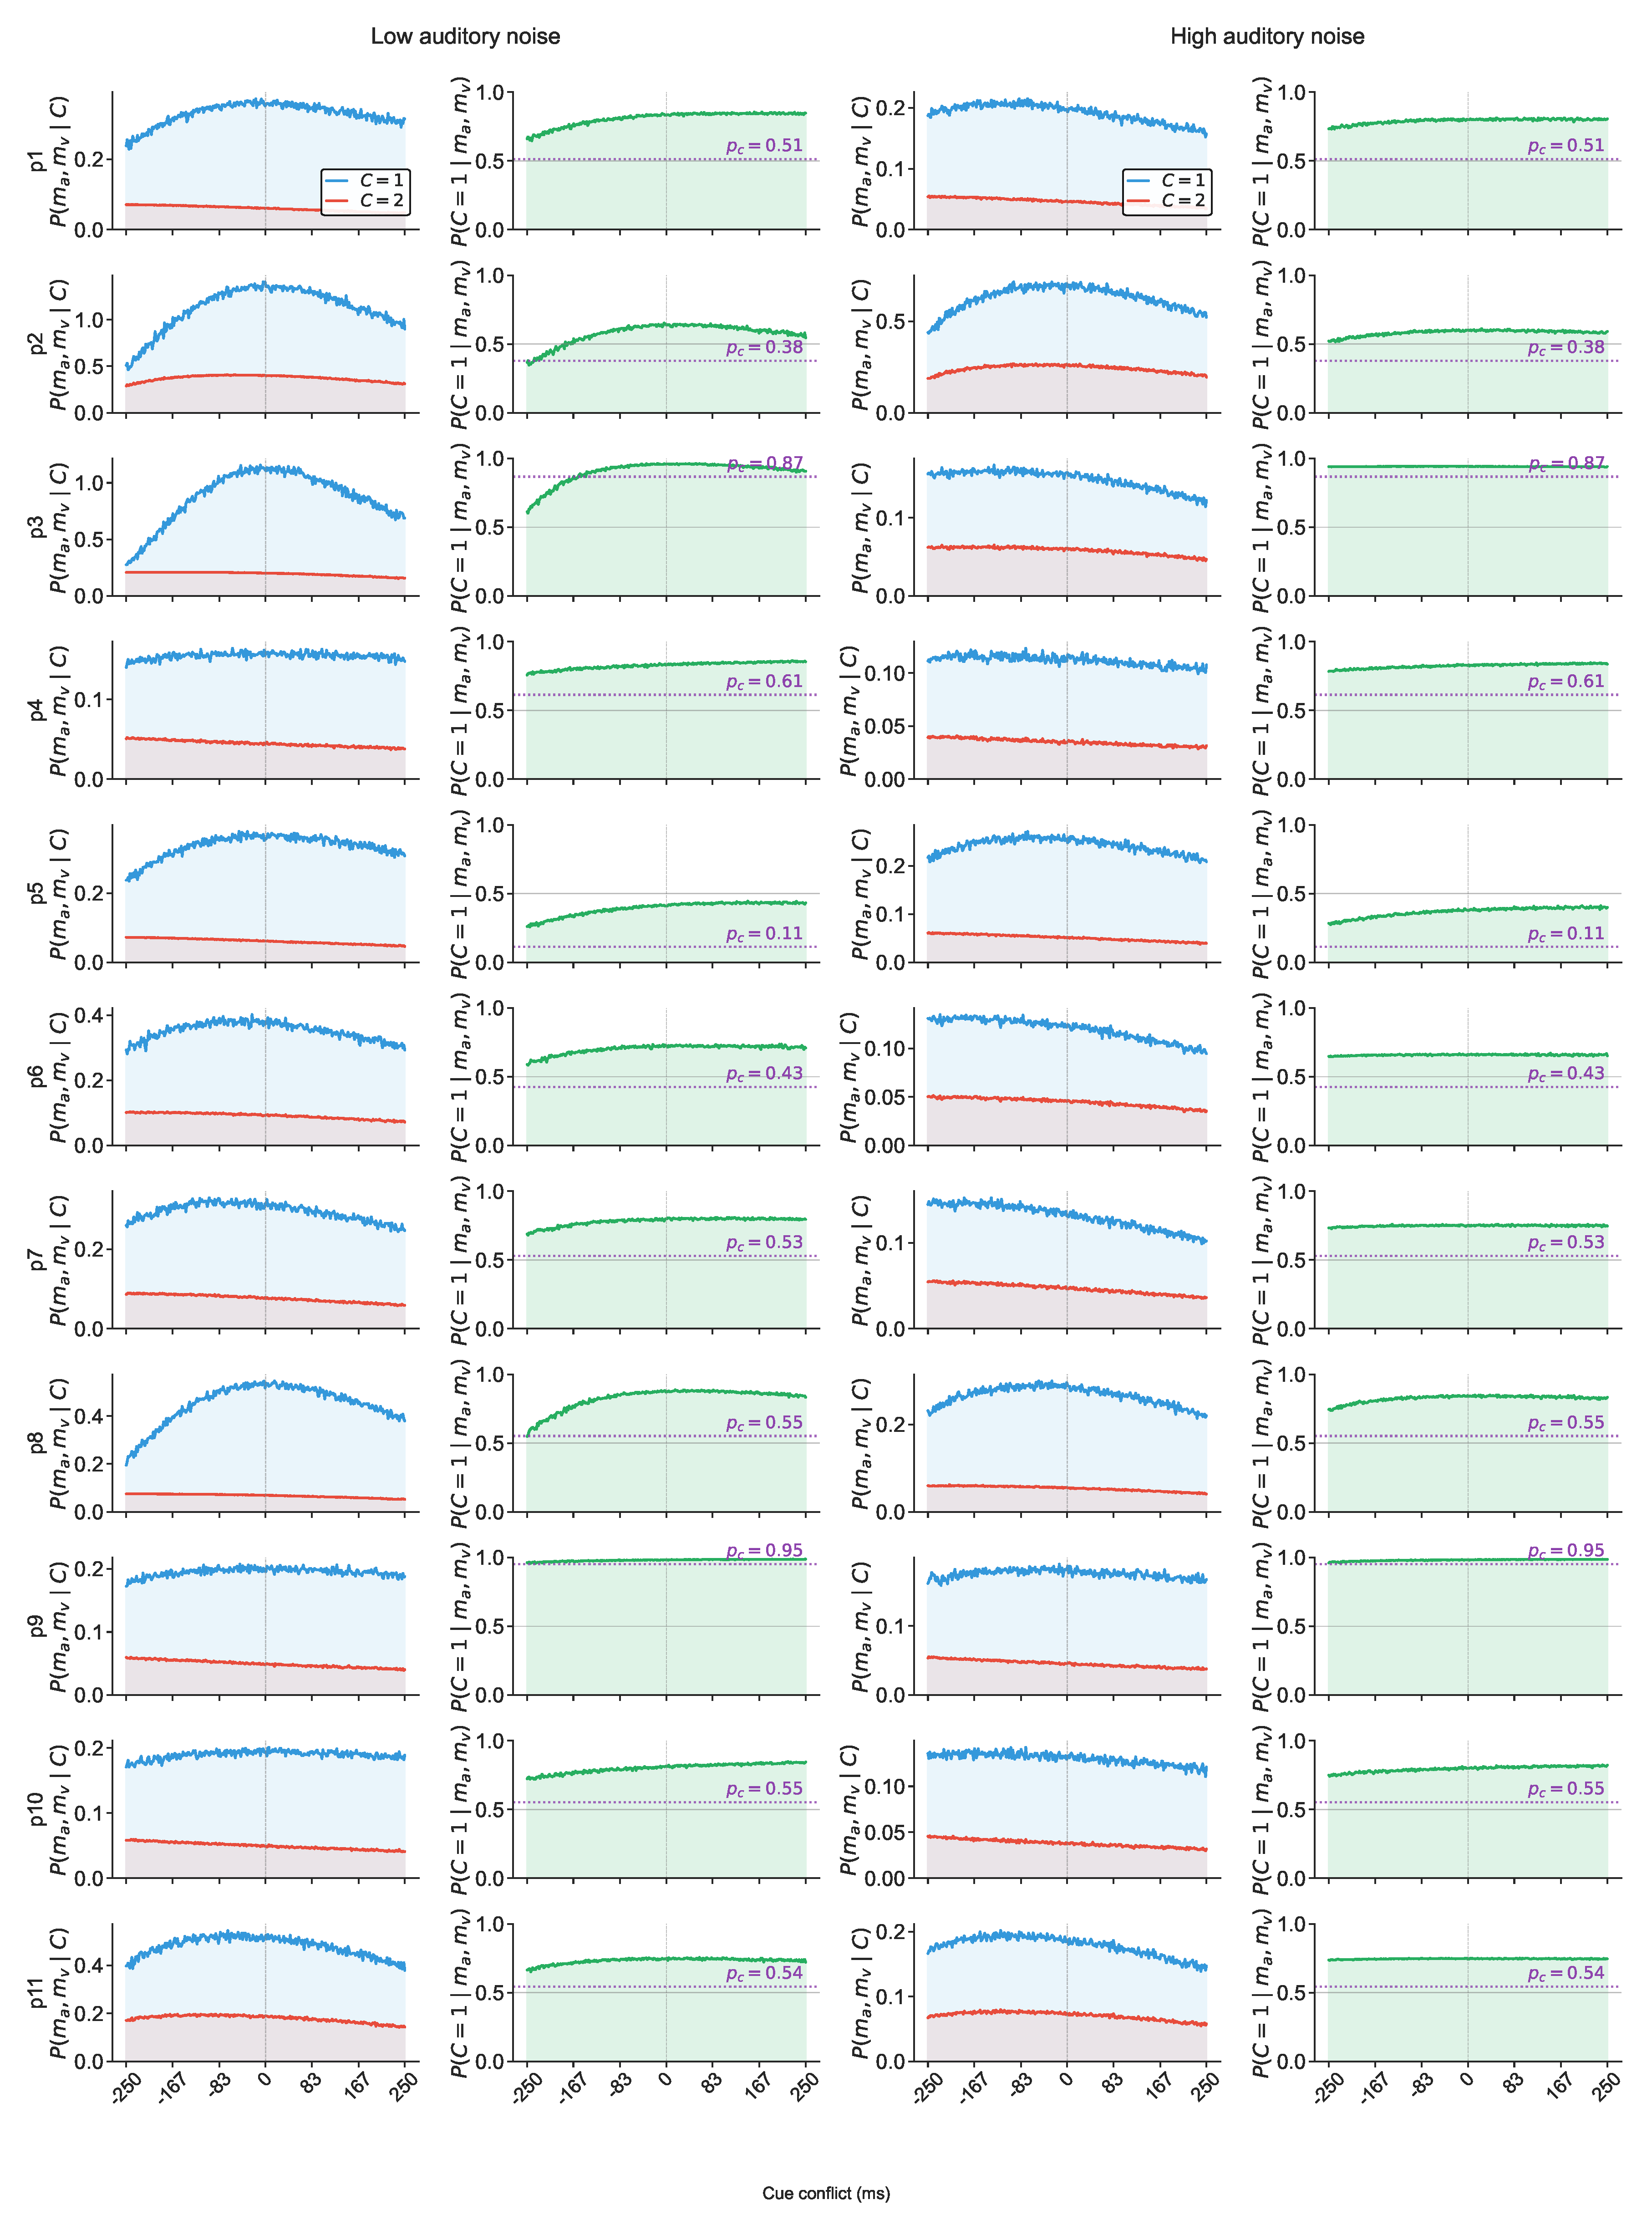
\includegraphics[width=0.85\linewidth]{assets/figures/posterior_overlay_per_subject_v3.pdf}
    \caption{\textbf{Log likelihoods and posterior probability of common cause for each participant.}
    Left two columns: low auditory noise; right two columns: high auditory noise. Columns 1 and 3: the log likelihood of the measurements under a common cause, $\log P(m_a, m_v \mid C{=}1)$ (blue), and under separate causes, $\log P(m_a, m_v \mid C{=}2)$ (red), are plotted on the same axes. Columns 2 and 4: the posterior probability of common cause, $P(C{=}1 \mid m_a, m_v)$, with the dotted line indicating the fitted prior $p_c$. Each row corresponds to one participant.}
    \label{fig:posterior_individual}
\end{figure}

\subsection{Posteriors and likelihoods of common causes}

To further illustrate how the causal-inference model interprets audiovisual conflict at the individual-participant level, Figure~\ref{fig:posterior_individual} shows the log-likelihoods of the common-cause and separate-causes hypotheses and the resulting posterior probability of common cause as a function of conflict magnitude under the fitted log-space causal-inference model. Across participants, the likelihood of a common cause generally remained comparable to or higher than that of separate causes, so the posterior probability of common cause stayed relatively high across the tested conflict range, particularly in the high-noise condition. All quantities were computed via Monte Carlo simulation using 2,000 samples per conflict level and participant-specific sensory-noise estimates ($\sigma_a$, $\sigma_v$) and common-cause prior ($p_c$) from the log-normal causal-inference model fit. Across participants,the posterior remains close to the prior for nearly all observers, indicating that the fitted parameters leave the causal-inference mechanism unable to distinguish common from separate causes at the conflict levels tested.


\subsection{Unimodal-derived predictions of bimodal uncertainty}

Figure~\ref{fig:optimalIntegrationComp} compares empirically observed audiovisual variability ($\sigma_{AV}$) with variability predicted under optimal reliability-weighted integration ($\sigma_{\mathrm{opt}}$), derived from unimodal sensory-noise estimates. 

Under the assumption of statistically optimal cue combination with independent Gaussian noise, the predicted audiovisual variance is given by
\begin{equation}
\sigma_{\mathrm{opt}}^2 = \frac{\sigma_a^2 \sigma_v^2}{\sigma_a^2 + \sigma_v^2}
= \frac{1}{J_a + J_v},
\end{equation}
where $\sigma_a$ and $\sigma_v$ denote auditory and visual noise, respectively, and $J_a = 1/\sigma_a^2$, $J_v = 1/\sigma_v^2$ are the corresponding precisions.

Observed audiovisual variability ($\sigma_{AV}$) was estimated by fitting psychometric functions to bimodal data. Predictions were computed separately for the high- and low-noise auditory conditions using the corresponding unimodal estimates ($\sigma_{a,h}$ and $\sigma_{a,l}$), and compared to the fitted bimodal variability.

Panels show results for each noise conditions. Each point corresponds to an individual participant (color-coded). The dashed unity line ($\sigma_{\mathrm{opt}} = \sigma_{AV}$) indicates perfect agreement between predicted and observed variability. Systematic deviations from this line reflect departures from optimal integration based solely on unimodal noise estimates.

\begin{figure}[H]
    \centering
    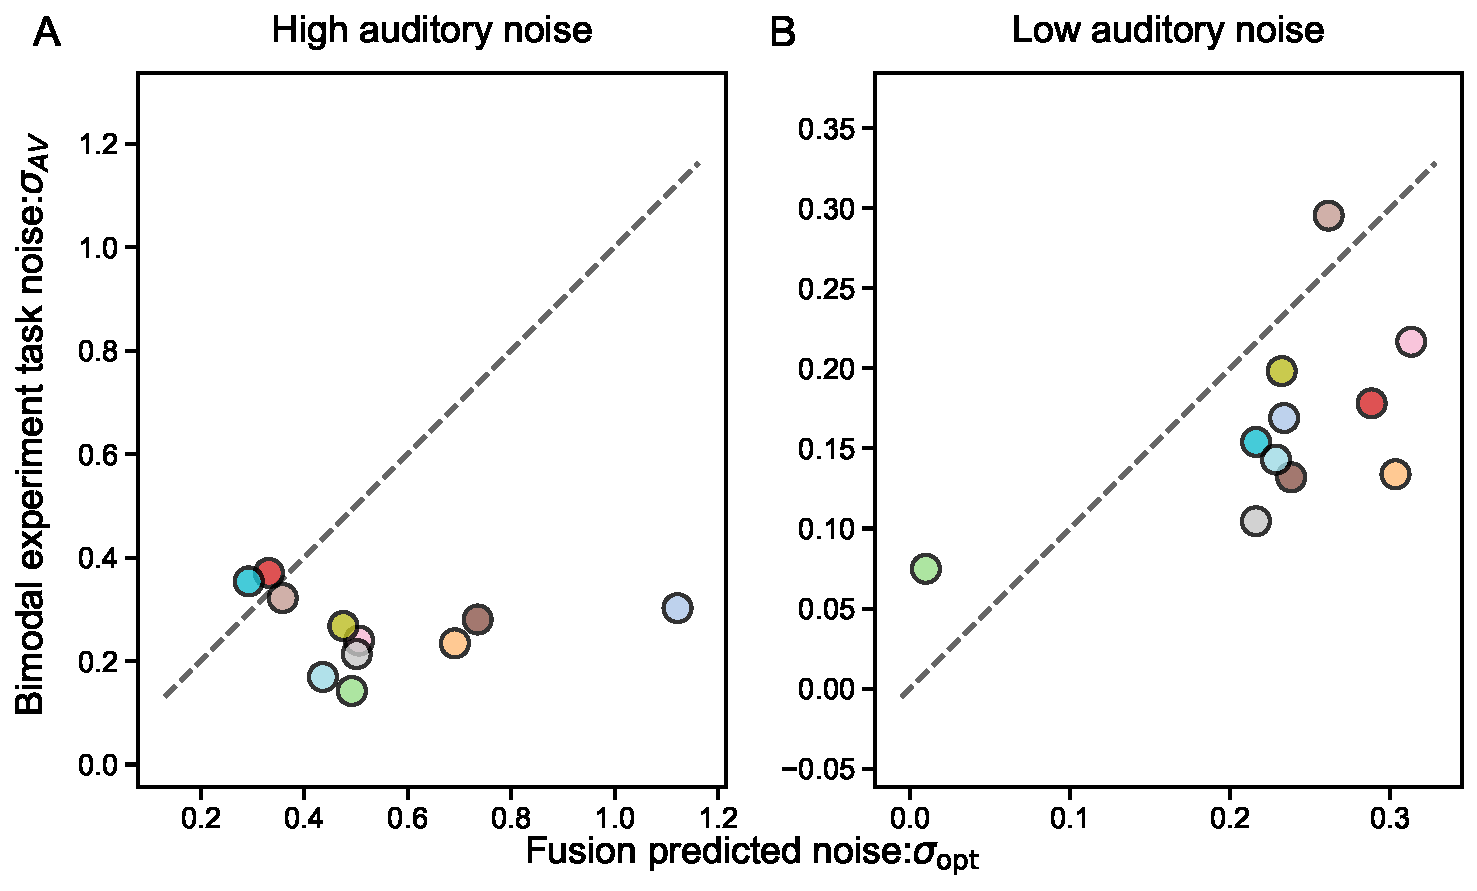
\includegraphics[width=1\linewidth]{assets/figures/optimal_integration_comparison.pdf}
    \caption{\textbf{Comparison of predicted optimal-integration variability with observed audiovisual variability.}
    Each panel compares empirically observed audiovisual variability ($\sigma_{AV}$; obtained by fitting psychometric functions to bimodal data, y-axis)
    with variability predicted by optimal reliability-weighted integration ($\sigma_{\mathrm{opt}}$, x-axis), computed from unimodal psychometric-fit noise estimates
    ($\sigma_{a,h}$ and $\sigma_{a,\ell}$ for auditory high- and low-noise conditions, and $\sigma_v$ for vision).
    Each point is one participant; the dashed line indicates equality ($\sigma_{\mathrm{opt}}=\sigma_{AV}$).}
    \label{fig:optimalIntegrationComp}
\end{figure}


Interestingly, observed audiovisual noise was substantially lower than the noise predicted by optimal reliability-weighted integration based on unimodal sensory estimates, particularly in the high auditory-noise condition. In several participants, bimodal uncertainty fell well below the unity line, indicating stronger precision than predicted from unimodal noise alone.

One possible explanation is that the visual stimulus in the bimodal task provided highly precise temporal anchors marking stimulus onset and offset. These visual transients may reduce temporal uncertainty beyond simple duration integration by improving the detection of the interval itself. As a result, auditory duration judgments in the bimodal task may benefit from additional temporal structure (precise cue for onset and offset of the event) that is absent in the unimodal auditory condition, leading to lower overall variability than predicted from unimodal noise estimates alone.

A second possibility is that sensory precision should not be expected to stay stationary across experiment and trials. The bimodal task involved substantially more trials and longer exposure to the stimulus structure, potentially leading to implicit training on temporal discrimination over time. If unimodal noise estimates reflect earlier performance, they may overestimate the effective sensory variability present during the bimodal experiment.

These findings suggest that unimodal-derived sensory noise parameters may not fully generalize to multisensory contexts, particularly when additional temporal cues are available.




\begin{figure}
    \centering
    
\includegraphics[width=1\linewidth]{assets/figures/empirical_confusion_3model.pdf}
    \caption {Model recovery. Validation of model identifiability through synthetic data analysis. For each of the three candidate models (rows), we generated 50 synthetic datasets using parameters sampled from the group-level distribution (mean $\pm$ SD from 11 participants). All models were then fit to each synthetic dataset, and the best-fitting model was determined by AIC. Row-normalized recovery rates show the proportion of times when data generated by one model was identified as coming from each of the three models. Values on the diagonal indicate successful recovery of the true generating model. The moderate values along the diagonal reveal important differences in model identifiability: probabilistic cue switching show good recovery, while averaging-based models (forced fusion, causal inference)show poor recovery, indicating that these models make similar predictions and are not discriminable using our behavioral data.}
    \label{fig:modelRecoveryResults}
\end{figure}

\subsection{Model recovery}

Model recovery is a crucial validation step that tests whether our model-comparison procedure can correctly identify the true data-generating model. This ensures that when we select a "best model" for real data, we're doing so reliably. 
To perform this analysis, after fitting each candidate model to the empirical data, we used the fitted parameter values to generate 50 synthetic datasets per model. Parameters were sampled from group-level distributions estimated from the 11 participants included in the main analyses. For each sampled parameter set, we simulated trial-by-trial responses according to the probabilities predicted by the generating model’s psychometric function. Each synthetic dataset matched the original experimental design (same stimulus conditions, trial counts, and structure). We then fit all candidate models to every simulated dataset and recorded their AIC values and the winning model.


The model-recovery results reveal substantial differences in identifiability across models (Figure~\ref{fig:modelRecoveryResults}). Recovery was strongest for the probabilistic cue switching strategy, which was correctly identified in 92\% of simulated datasets, indicating that this model generates relatively distinctive behavioral predictions. Recovery for the Forced fusion model was more moderate (64\%), with appreciable confusion with causal inference model. In contrast, causal inference showed poor mutual discriminability which is recovered and equally confused with forced fusion model at 44\%. This pattern suggests that only the probabilistic cue switching model generates distinguishable behavioral signatures.

%%% --- adding this: model-recovery asymmetry (cue-switching preference is not spurious flexibility) ---
% Reproducibility: grid_recovery_summary.ipynb, section 6 (three-model recovery) over model_recovery_results_group_logfixed_ns1_nsim2000/group_*_model_recovery.json (off-diagonal AIC-winner counts).

Importantly, the high recovery of the cue-switching model did not reflect a general tendency to over-select the most flexible model. Cue switching was selected for only $6$ of $50$ datasets generated by forced fusion and $6$ of $50$ generated by causal inference, but for $46$ of $50$ datasets that it generated itself. Its preference in the empirical data therefore reflects a genuine, recoverable behavioral signature rather than spurious model flexibility.
%%% --- end added section ---


\begin{figure}
    \centering
    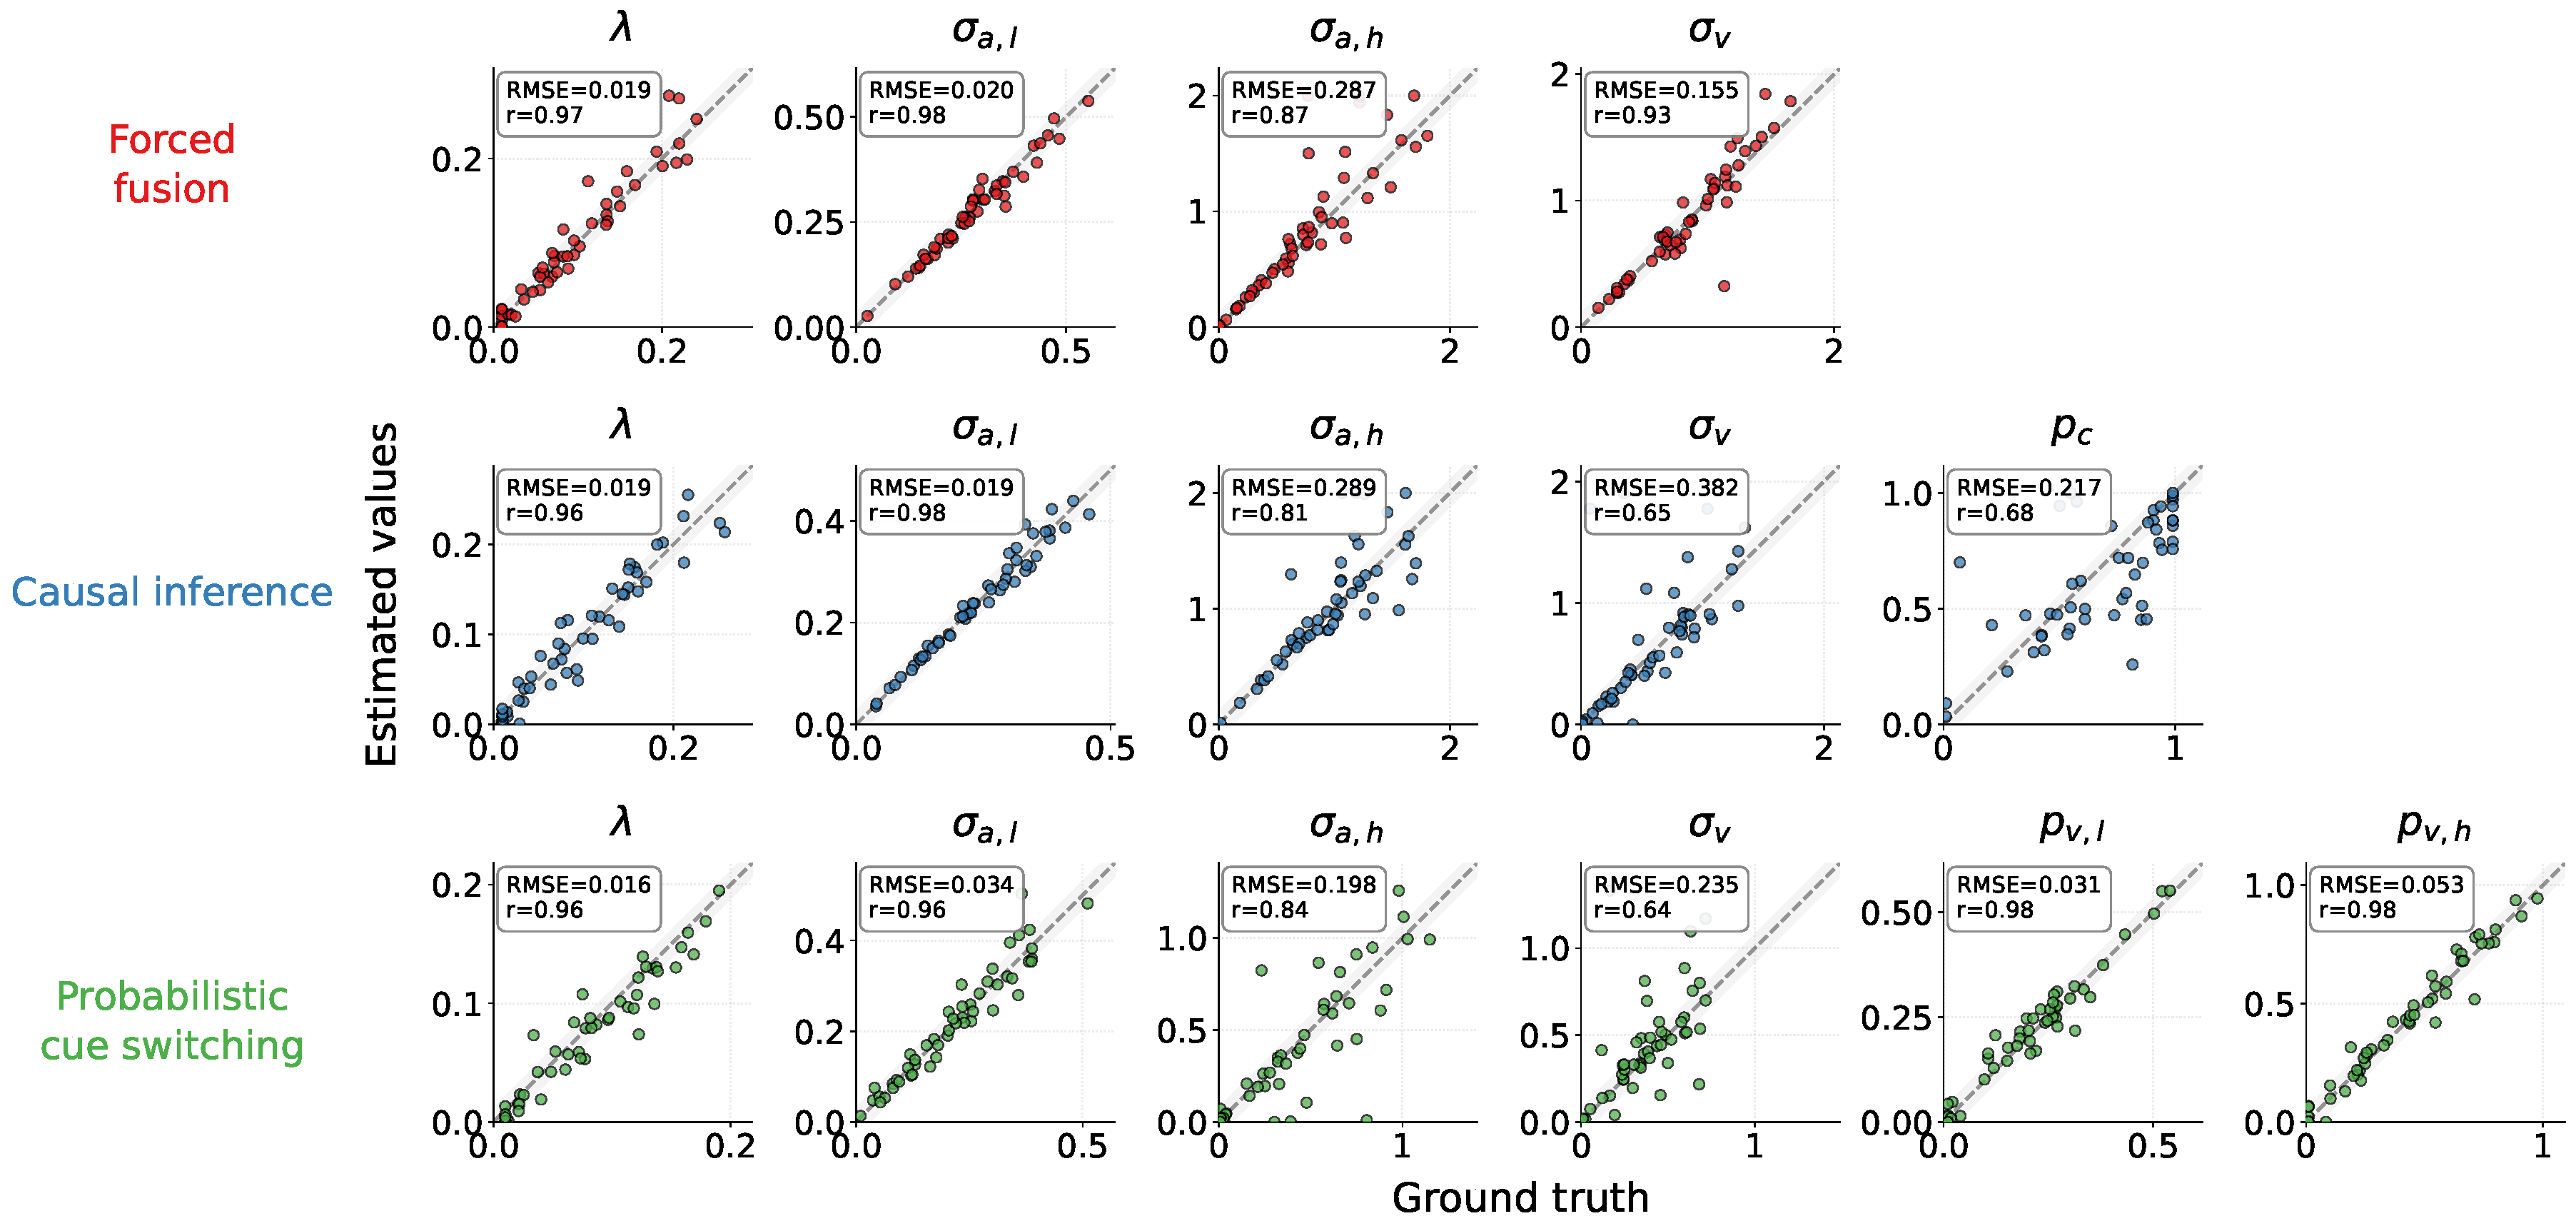
\includegraphics[width=1\linewidth,height=0.58\textheight,keepaspectratio]{assets/figures/emprical_parameter_recovery_nIter_50.pdf}
    \caption{\textbf{Parameter-recovery analysis for model validation.} Each row corresponds to a generative model and each column to a model parameter. Synthetic datasets ($N = 50$) were generated from fitted group-level parameter distributions and refit with the same model. Scatter plots show true versus recovered parameter values; dashed diagonals indicate perfect recovery and gray bands show a $\pm 5\%$ tolerance region. Insets report Pearson correlation ($r$) and RMSE. Sensory-noise and lapse parameters were generally well recovered, whereas causal-prior and switching parameters were less constrained.}
    \label{fig:parameterRecovery}
\end{figure}

\subsection{Parameter recovery}

Using the same synthetic datasets, we also conducted a parameter-recovery analysis to confirm that each model's parameters can be reliably recovered from data generated by that model (Figure~\ref{fig:parameterRecovery}). The parameter-recovery results (Figure~\ref{fig:parameterRecovery}) demonstrate that model parameters are, in general, well identified. Across models, key sensory-noise parameters ($\sigma_{a,l}$, $\sigma_{a,h}$, $\sigma_v$) and the lapse rate ($\lambda$) show high correlations between true and recovered values and cluster tightly around the identity line, indicating reliable estimation. In contrast, parameters governing causal inference or strategy selection (e.g., $p_c$ and switching probabilities) exhibit lower correlations and higher variability, reflecting weaker identifiability. This pattern is consistent with the model-recovery results: parameters that strongly shape the psychometric function (e.g., sensory noise) are robustly recovered, whereas the causal relation ($p_c$) parameters was harder to estimate precisely. Importantly, the overall success of parameter recovery confirms that the fitting procedure can reliably capture the main computational components of each model, even in cases where models themselves are difficult to distinguish at a fine-grained level.This dissociation suggests that limitations in model recovery arise primarily from overlapping model predictions rather than from failures of parameter estimation.


%%% ----------------------------%%% ----------------------------

\subsection{Extended simulations across sensory-noise and conflict regimes}

To assess when the candidate models should be expected to become distinguishable, and under which conditions the hypotheses about cue integration could be disentangled, we performed an extended model-recovery analysis across simulated sensory-noise and conflict sampling regimes. We simulated datasets from the three candidate models while varying both the sensory-noise range and the maximum audiovisual conflict. Four sensory-noise regimes were sampled from: very low noise, $\sigma_a,\sigma_v \sim U[0.01,0.20]$; low noise, $\sigma_a,\sigma_v \sim U[0.20,0.40]$; medium noise, $\sigma_a,\sigma_v \sim U[0.30,0.70]$; and an empirical regime based on the range of fitted sensory-noise parameters. For the synthetic regimes, auditory and visual sensory noise parameters were sampled from the same range.

The grid recovery analysis should be read as a map of model identifiability across possible experimental regimes. Each panel shows how often the generating model was recovered after refitting simulated datasets with all three candidate models. Higher diagonal values indicate better model recovery, whereas off-diagonal values indicate systematic confusions between models. Moving from left to right increases sensory uncertainty, and moving from the top row to the bottom row reduces the maximum conflict range from $0.45\,\mathrm{s}$ to $0.25\,\mathrm{s}$.

This analysis shows that model discriminability depends strongly on both sensory noise and the tested range of audiovisual conflicts. Recovery was generally best when sensory noise was low and the conflict range was wide, and poorest when sensory noise was higher and the conflict range was narrow. Importantly, the empirical recovery panel shows that the experimentally observed regime was one in which Forced fusion and Causal inference were difficult to distinguish, whereas Probabilistic Cue Switching remained relatively identifiable.

Model recovery generally improved as sensory noise decreased and as the maximum conflict range increased from $0.25\,\mathrm{s}$ to $0.45\,\mathrm{s}$. This pattern suggests that larger audiovisual discrepancies and lower sensory uncertainty provide more diagnostic information for distinguishing between integration strategies. For the experimentally tested conflict range, where the maximum conflict was $0.25\,\mathrm{s}$, recovery remained more limited, especially for distinguishing forced fusion from causal inference. However, probabilistic cue switching remained comparatively identifiable in the empirical recovery analysis.

One exception was that, under the wider $0.45\,\mathrm{s}$ conflict range, the very-low-noise regime showed slightly lower mean recovery than the low-noise regime. This may reflect a regime in which model predictions become less graded across conflict levels because large conflicts combined with very precise sensory estimates strongly favor segregated or cue-specific responses. Thus, while lower sensory noise generally improves model identifiability, the most informative regime is not necessarily the lowest-noise regime, but one in which model predictions remain sufficiently distinct across the tested conflict values.

These simulations indicate that model identifiability is strongly constrained by sensory uncertainty and conflict magnitude. In particular, the empirical recovery analysis showed substantial confusion between Forced Fusion and Causal Inference, whereas Probabilistic Cue Switching remained highly identifiable ($92\%$ correct recovery). Thus, within the experimentally tested conflict range and observed sensory-noise levels, competing integration models can generate highly similar behavioral predictions.

%%% ----------------------------%%% ----------------------------

% We simulated the models by using 4 different parameter sampling range to test at which theoretical sensory noise levels would these models be distinguishable from each other. We simulated the models across four sensor noise paramater sampling ranges (3 constrained ranges and the empirical range as a baseline: "very low - $\sigma_a$: [0.01–0.20], "low $\sigma_b$:" [0.20–0.40], "medium $\sigma_c$:" [0.30–0.70], and "empirical $\sigma_d$:"[$\sigma_a$: 0.11–0.48, $\sigma_v$:0.14–1.60]). For the simulated model recoveries we selected both the auditory sensory noise and visual sensory noise from same sampling range. When we analyse the confusion of these models we see that the overall recovery rate in general increased at each step of lowering the sensory noise paramater sampling range from emprical(high) till low sensory noise sampling ranges. Also the recovery rate increased for extended unreasonable maximum conflict range experiment simulations from 0.25s maximum conflict to 0.45s conflict range condition. Interestingly for the 0.45s max conflict condition "very low" sensory noise sampled simulation had a lower recovery rate than the "low" sensory noise sampled simulation condition. We speculate that this result is due to almost flat estimate at each conflict condition where the model predicts no common cause, as can be said as no fusion, as can be said as always selects the audtiory estimate. Tough for experimentaly tested conflict range (0.25s of maximum conflict) to reach the highest recovery rate (mean 77\%) simulations show us that we would need to have the lowest sensory noise sampling range.  

\begin{figure}[H]
    \centering
    
\includegraphics[width=1\linewidth,height=1\textheight,keepaspectratio]{assets/figures/grid_three_model_confusion_matrices.pdf}
    \caption{\textbf{Model recovery across sensory-noise and conflict regimes.} Confusion matrices for the three candidate models: Forced Fusion (FF), Causal Inference (CI), and Probabilistic Cue Switching (PCS). Rows indicate the generating model and columns indicate the recovered model selected by AIC. Cell values show row-normalized recovery percentages, with diagonal entries corresponding to correct recovery. Panels compare four sensory-noise regimes and two maximum conflict ranges. The top row uses $\mathrm{conflict}_{\max}=0.45\,\mathrm{s}$, whereas the bottom row uses $\mathrm{conflict}_{\max}=0.25\,\mathrm{s}$. Synthetic sensory-noise regimes were defined as $\sigma_a,\sigma_v\sim U[0.01,0.20]$, $U[0.20,0.40]$, and $U[0.30,0.70]$. The empirical panel highlighted in red was computed from datasets simulated using the fitted participant-level parameters and refitted with all candidate models. Recovery generally decreased with increasing sensory noise and narrower conflict ranges. Under the empirical parameter regime, PCS showed high recovery, whereas FF and CI showed greater mutual confusability.}
    \label{fig:gridModelRecovery}
\end{figure}


One implication of this analysis is that larger audiovisual conflicts could, in principle, improve model discriminability by producing stronger differences in likelihood and AIC across models. However, substantially increasing the conflict range was not feasible for the present experiment. First, audiovisual conflicts were defined relative to each participant's subjective audiovisual bias, so that auditory and visual durations were adjusted to produce approximately matched perceived durations. For three participants with a positive visual-duration bias, this calibration limited the range of negative conflicts that could be presented while keeping stimulus durations within the intended range. Second, extending the maximum conflict to approximately $0.45\,\mathrm{s}$ would have produced highly unusual audiovisual duration pairings. For example, at a $+0.45\,\mathrm{s}$ conflict, the visual stimulus would approach $0.95\,\mathrm{s}$, which may alter sensory uncertainty and produce behavior outside the regime targeted by the experiment. Thus, while larger conflicts may improve theoretical model recovery, they would also change the perceptual and experimental context being modeled. 




\bibliographystyle{apalike}
\bibliography{elife-sample}

\end{document}
